\documentclass[12pt]{article}
% Load packages
\usepackage{url}  % Formatting web addresses
\usepackage{ifthen}  % Conditional
\usepackage{multicol}   %Columns
\usepackage[utf8]{inputenc} %unicode support
\usepackage{amsmath}
\usepackage{amssymb}
\usepackage{epsfig}
\usepackage{epstopdf}
\usepackage{graphicx}
\usepackage[margin=0.1pt,font=footnotesize,labelfont=bf]{caption}
\usepackage{setspace}
%\usepackage{longtable}
\usepackage{colortbl}
%\usepackage{palatino,lettrine}
%\usepackage{times}
%\usepackage[applemac]{inputenc} %applemac support if unicode package fails
%\usepackage[latin1]{inputenc} %UNIX support if unicode package fails
\usepackage[wide]{sidecap}
%\usepackage[authoryear,round,comma,sort&compress]{natbib}
\usepackage[round,sort,comma,numbers,sort&compress]{natbib}
%\usepackage[authoryear,round]{natbib}
\usepackage{supertabular}
\usepackage{simplemargins}
\usepackage{fullpage}
\usepackage{comment}
\usepackage{lineno}
%\usepackage{chicago}
\usepackage{textcomp}
\usepackage{multirow}
\usepackage{amsmath}
\usepackage[linesnumbered,lined,boxed,commentsnumbered]{algorithm2e}
\DeclareMathOperator*{\argmin}{\arg\!\min}

\usepackage{algorithm2e}
\usepackage{algpseudocode}
%\usepackage[space]{cite}
\urlstyle{rm}

%\textwidth = 6.50 in
%\textheight = 9.5 in
%\oddsidemargin =  0.0 in
%\evensidemargin = 0.0 in
%\topmargin = -0.50 in
%\headheight = 0.0 in
%\headsep = 0.25 in
%\parskip = 0.15in
%\linespread{1.75}
\doublespace

%\bibliographystyle{chicago}
\bibliographystyle{plos2009}

\makeatletter
\renewcommand\subsection{\@startsection
	{subsection}{2}{0mm}
	{-0.05in}
	{-0.5\baselineskip}
	{\normalfont\normalsize\bfseries}}
\renewcommand\subsubsection{\@startsection
	{subsubsection}{2}{0mm}
	{-0.05in}
	{-0.5\baselineskip}
	{\normalfont\normalsize\itshape}}
\renewcommand\section{\@startsection
	{subsection}{2}{0mm}
	{-0.2in}
	{0.05\baselineskip}
	{\normalfont\large\bfseries}}
\renewcommand\paragraph{\@startsection
	{paragraph}{2}{0mm}
	{-0.05in}
	{-0.5\baselineskip}
	{\normalfont\normalsize\itshape}}
\makeatother

%Review style settings
%\newenvironment{bmcformat}{\begin{raggedright}\baselineskip20pt\sloppy\setboolean{publ}{false}}{\end{raggedright}\baselineskip20pt\sloppy}

%Publication style settings

% Single space'd bib -
\setlength\bibsep{0pt}

\renewcommand{\rmdefault}{phv}\renewcommand{\sfdefault}{phv}
\newcommand{\norm}[1]{\left\lVert#1\right\rVert}

% Change the number format in the ref list -
\renewcommand{\bibnumfmt}[1]{#1.}

% Change Figure to Fig.
\renewcommand{\figurename}{Fig.}

% Begin ...
\begin{document}
\begin{titlepage}
{\par\centering\textbf{\Large {Reduced order modeling and analysis of the human complement system}}}
\vspace{0.05in}
{\par \centering \large{Adithya Sagar, Wei Dai$^{\#}$, Mason Minot$^{\#}$, and Jeffrey D. Varner$^{*}$}}
\vspace{0.10in}
{\par \centering {School of Chemical and Biomolecular Engineering}}
{\par \centering {Cornell University, Ithaca NY 14853}}
\vspace{0.1in}
{\par \centering \textbf{Running Title:}~A reduced order model of complement}
\vspace{0.1in}
{\par \centering \textbf{To be submitted:}~\emph{PLoS~ONE}}
\vspace{0.5in}
{\par \centering $^{\#}$ Denotes equal contribution}
\vspace{0.1in}
{\par \centering $^{*}$Corresponding author:}
{\par \centering Jeffrey D. Varner,}
{\par \centering Professor, School of Chemical and Biomolecular Engineering,}
{\par \centering 244 Olin Hall, Cornell University, Ithaca NY, 14853}
{\par \centering Email: jdv27@cornell.edu}
{\par \centering Phone: (607) 255 - 4258}
{\par \centering Fax: (607) 255 - 9166}
\end{titlepage}
\date{}
\thispagestyle{empty}
\pagebreak
%%%%%%%%%%%%%%%%%%%%%%%%%%%%%%%%%%%%%%%%%%%%%%%%%%%%%%%%%%%%%%%%%%%%%%%%%%%%%%%%%%%%%%%%%%%%%%%%%%%%%%%%%%%
%%%%%%%%%%%%%%%%%%%%%%%%%%%%%%%%%%%%%%%%%%%%%%%%%%%%%%%%%%%%%%%%%%%%%%%%%%%%%%%%%%%%%%%%%%%%%%%%%%%%%%%%%%%
\section*{Abstract}
Complement is an important pathway of innate immunity which plays a significant role in inflammation, and many other disease processes.
However, despite its importance, there has been a paucity of validated mathematical models of complement activation.
In this study, we developed an ensemble of experimentally validated reduced order complement models.
The modeling approach combined ordinary differential equations with logical rules to produce a complement model with a limited number of equations and parameters.
The reduced order model,  which described the lectin and alternative pathways, consisted of 18 differential equations with 28 parameters.
Thus, the model was an order of magnitude smaller and included more pathways than comparable models in the literature.
We estimated an ensemble of model parameters from \textit{in~vitro} time series measurements of the C3a and C5a complement proteins.
Subsequently, we validated the model on unseen C3a and C5a measurements that were not used for model training.
Despite its small size, the model was surprisingly predictive.
After validation, we performed global sensitivity and robustness analysis to estimate which parameters and species
controlled model performance. These analyses suggested complement was robust to any single therapeutic intervention.
The only intervention that consistently reduced C5a formation for all cases was a dual-knockdown of both C3 and C5.
Taken together, we developed a reduced order complement model that was computationally inexpensive,
and could easily be incorporated into pre-existing or new pharmacokinetic models of immune system function.
The model described experimental data, and predicted the need for multiple points of therapeutic intervention to disrupt complement activation.

% We used this framework to capture the dynamics of C3a and C5a formation from the lectin and alternative pathways.
%and includes more pathways than comparable purely ODE models in the literature. We estimated the model parameters from in vitro human complement time-course experiments of C3a and C5a from Morad and coworkers, in the presence and absence of zymosan, and without the classical pathway.
%We then compared the model predictions with C3a and C5a data sets, for alternative and lectin pathway dynamics, that were not used for model training. Once validated, we performed sensitivity analysis on the model to estimate which parameters were critical to model performance in several conditions. The reduced order hybrid approach produced a surprisingly predictive human complement model, much similar to the study on human coagulation using the same modeling framework \cite{sagar2015dynamic}. Taken together, the combined analysis of alternate and lectin pathways along with the incorporation of the downstream reactions involving C5 convertase elucidated new insight into roles of governing parameters that mediate the complement system. Deeply understanding how the main governing parameters change with respective to the different combinations of pathway activation will greatly aid in development of drugs for strategic therapeutic targets. Due to the low computational cost relative to the existing models and accuracy of our predictions, we believe that our reduced order complement network is the first step towards building a computation toolbox for treatment analysis or clinical screening in the medical field.


\vspace{0.1in}
{\noindent \textbf{Keywords:}~Complement system, systems biology, reduced order models, biochemical engineering}

\pagebreak

\setcounter{page}{1}

% Uncomment in production -
\linenumbers


\section*{Introduction}



%Complement is a central part of innate immunity and plays a very significant role in regulating the inflammatory response. It was first discovered in the 1890s where it was found to 'complement' the bactericidal activity of natural antibodies. Complement is mediated through a set of approximately 30-35 soluble and cell surface proteases \cite{}. The central process in complement activation involves the formation of Membrane Attack Complex (MAC) and a protein called C5a. Complement activation takes places through three different pathways: the alternate, the classical and the lectin. Each of these pathways involves a different initiator signal that leads to the formation of a serine protease called C5 convertase which cleaves an inactive protein called C5 to form C5a and C5b. The classical pathway is triggered when antibodies form complexes with foreign antigens or other pathogens. A multimeric protein complex C1 binds to the antigen-antibody complex and undergoes a conformational change. This activated complex cleaves proteins C4 and C2 to C4a, C4b, C2a and C2b respectively. C4a and C2b combine to form a protease C4bC2a also known as the classical C3 convertase. The lectin pathway is initiated through the binding of L-ficolin or Mannose Binding Lectin (MBL) to the carbohydrates on the surfaces of bacterial pathogens. This bound complex in turn cleaves C4 and C2 and leads to the production of C4bC2a. The alternate pathway involves a 'tickover' mechanism in which a protein called C3 is hydrolyzed to form C3b. In presence of foreign pathogens C3b binds to these surfaces and recruits  additional factors called factor B and factor D that lead to the formation of alternate C3 convertase - C3bBb. The formation of classical and alternate C3 convertases on bacterial surfaces is followed by the formation of proteases called C5 convertases. The classical and alternate C3 convertases recruit C3, Factor B and Factor D to form classical C5 convertase (C4bC2aC3b) and alternate C5 convertase (C3bBbc3B) respectively. The C5 convertases then cleave C5 to form C5a and C5b respectively. 	The cleavage of C5 is followed by a series of sequential cleavages of proteins C6, C7, C8 and C9 that combine with C5b to form the MAC complex. The activation of complement and formation of C5a and MAC complex is regulated at different points through a number of plasma and host cell proteins. The initiation of the classical pathway through the attachment of C1 to an antibody is controlled by the C1 Inhibitor (C1-Inh), a protease inhibitor belonging to the serpin superfamily. C1-Inh irreversibly binds to and deactivates the active subunits of component C1 to prevent spontaneous fluid phase and chronic activation of complement \cite{walker1995complement}. The serum and host-tissue regulation of the upstream elements of the complement system is also achieved through the binding of C4 binding protein (C4BP) to C4b and through the binding of factor H to C3b \cite{blom2001structural}. These proteins are also capable of binding their respective components in the convertase form. Membrane cofactor protein (MCP or CD46) possesses a cofactor activity for C4b and C3b, which protects the host from self-activation of complement \cite{riley2004cd46}.  Decay accelerating factor (DAF or CD55) is able to recognize and dissociate both convertases \cite{lukacik2004complement}. MAC is inhibited by vitronectin and clusterin in the plasma and CD59 at the host surface.
%Proteins C3a, C4a, and C5a are inactivated or reduced in activity by carboxypeptidase-N \cite{liszewski1995control}.
%The system's involvement in a variety of beneficial regulatory processes coupled with the role it can play in disease makes it important to understand complement in a more holistic perspective.
%Given the complexity of complement and its interactions with other networks it is unfeasible and computationally expensive to build such large mechanistic models. In addition is much more difficult to experimentally interrogate the response of various complement proteins under different conditions. This also presents with the problem of estimation of a large number of parameters with little or no experimental data. Thus there exists a need to reduce the mechanistic complexity while capturing dynamics of complement accurately.

Complement is an important pathway in innate immunity. It plays a significant role in inflammation, host defense as well as many disease processes.
Complement was discovered in the late 1880s where it was found to 'complement' the bactericidal activity of natural antibodies \cite{OG_COMPLEMENT_REF}.
However, research over the past decade has shown the importance of complement extends well beyond innate immunity.
For example, complement contributes to tissue homeostasis by inducing growth factors involved in tissue repair \cite{ricklin2010complement}.
Complement malfunctions have been linked with several diseases including Alzheimers, glaucoma, Parkinson's disease, multiple sclerosis, schizophrenia, rheumatoid arthritis and sepsis \cite{ricklin2007complement, rittirsch2008harmful}.
Complement can also play both a positive and negative role in certain cancers; attacking tumor cells with altered surface proteins in some cases, while potentially contributing to tumor growth in others \cite{sarma2011complement, ricklin2013complement}.
Several other important biochemical networks are integrated with complement including the coagulation cascade, the autonomous nervous system and the ability to regulate inflammation \cite{ricklin2013complement}. Thus, complement is an important system involved in a variety of both beneficial and potentially harmful functions in the body.

Complement is mediated by over 30 soluble and cell surface proteins that are present as inactive forms in the circulation \cite{walport2001complement}.
The central output of complement activation is the formation of the Membrane Attack Complex (MAC) and a key protein called C5a.
The membrane attack complex forms transmembrane channels which disrupt the cell membrane of targeted cells, leading to cell lysis and death.
The C5a protein acts as a bridge between innate and adaptive immunity, and plays an important role in regulating inflammation and coagulation \cite{sarma2011complement}.
Complement activation takes places through three pathways: the alternate, the classical and the lectin binding pathway.
Each of these pathways involves a different initiator signal which leads to a cascade of downstream events in the complement system.
The classical pathway is triggered when antibodies form complexes with foreign antigens or other pathogens.
A multimeric protein complex C1 binds to the antigen-antibody complex and undergoes a conformational change.
This activated complex then cleaves complement proteins C4 and C2 into C4a, C4b, C2a and C2b respectively.
The C4a and C2b fragments combine to form the C4bC2a protease, also known as the classical C3 convertase.
The lectin binding pathway is initiated through the binding of L-ficolin or Mannose Binding Lectin (MBL) to carbohydrates on the surfaces of bacterial pathogens.
This bound complex in turn cleaves C4 and C2, leading to the formation of C4bC2a.
The alternate pathway involves a 'tickover' mechanism in which complement protein C3 is hydrolyzed to form C3b.
In the presence of pathogens, the C3b fragment binds foreign surfaces and recruits the additional proteins, factor B and factor D, which lead to the formation of C3bBb, the alternate C3 convertase \cite{pangburn1984alternative}.
The formation of classical and alternate C3 convertases on bacterial surfaces is followed by the formation of proteases called C5 convertases.
The classical and alternate C3 convertases recruit C3, Factor B and Factor D to form the classical C5 convertase (C4bC2aC3b), and alternate C5 convertase (C3bBbc3B) respectively.
The C5 convertases then cleave C5 to form the C5a and C5b fragments.
The cleavage of C5 is followed by a series of sequential cleavage steps involving the C6, C7, C8 and C9 complement proteins
which combine with C5b to form the membrane attack complex \cite{ricklin2010complement}.

Complement activation is regulated by many plasma and host cell proteins.
The initiation of the classical pathway via complement protein C1 is controlled by the C1 Inhibitor (C1-Inh), a protease inhibitor belonging to the serpin superfamily.
C1-Inh irreversibly binds to and deactivates the active subunits of C1, preventing spontaneous fluid phase and chronic activation of complement \cite{walker1995complement}.
Regulation of the upstream elements of complement is also achieved through the interaction of the C4 binding protein (C4BP) with C4b, as well as
through the interaction of factor H with C3b \cite{blom2001structural}.
These regulatory proteins are also capable of binding their respective targets while they are bound in convertase complexes.
Membrane cofactor protein (MCP or CD46) possesses a cofactor activity for C4b and C3b, which protects the host from self-activation of complement \cite{riley2004cd46}.
Delay accelerating factor (DAF or CD55) is also able to recognize and dissociate both C3 and C5 convertases \cite{lukacik2004complement}.
Carboxypeptidase-N, a well known inflammation regulator, cleaves carboxyl-terminal arginines and lysines of the complement proteins C3a, C4a, and C5a rendering them inactive \cite{liszewski1995control}. Lastly, the assembly of the MAC complex is inhibited by vitronectin and clusterin in the plasma, and CD59 at the host surface \cite{chauhan2006presence,zewde2016quantitative}.
Thus, there are many points of control which influence complement activation across the three activation pathways.

Developing quantitative mathematical models of complement could be crucial to understanding its role in the body.
Traditionally, complement models have been formulated as systems of linear or non-linear ordinary differential equations (ODEs).
For example, Hirayama et al. modeled the classical complement pathway as a system of linear ODEs \cite{hirayama1996linear},
while Korotaevskiy and co-workers modeled the classical, lectin and alternate pathways as a system of non-linear ODEs \cite{korotaevskiy2009non}.
More recently, large mechanistic models of sections of complement have also been proposed.
For example, Liu et al. analyzed the formation of the classical and lectin C3 convertases, and the regulatory role of C4BP using a system of 45 non-linear ODEs with 85 parameters \cite{liu2011computational}.
Recently, Zewde and co-workers constructed a detailed mechanistic model of the alternative pathway which consisted of 107 ODEs and 74 kinetic parameters and delineated
the complement response of the host and pathogen \cite{zewde2016quantitative}.
However, these previous modeling studies involved little experimental validation.
Thus, while these models are undoubtably important theoretical tools, it is unclear if they can describe or quantitatively predict experimentally validated complement dynamics.
The central challenge is the estimation of model parameters from experimental data.
Unlike other important cascades, such as coagulation for which there are well developed experimental tools and many publicly available data sets,
the data for complement is relatively sparse. Missing or incomplete data sets, and limited quantitative data make the identification of mechanistic complement models difficult.

In this study, we developed an ensemble of experimentally validated reduced order complement models.
The modeling approach combined ordinary differential equations with logical rules to produce a complement model with a limited number of equations and parameters.
The reduced order model,  which described the lectin and alternative pathways, consisted of 18 differential equations with 28 parameters.
Thus, the model was an order of magnitude smaller and included more pathways than comparable mathematical models in the literature.
We estimated an ensemble of model parameters from \textit{in~vitro} time series measurements of the C3a and C5a complement proteins.
Subsequently, we validated the model on unseen C3a and C5a measurements that were not used for model training.
Despite its small size, the model was surprisingly predictive.
After validation, we performed global sensitivity and robustness analysis to estimate which parameters and species
controlled model performance. These analyses suggested complement was robust to any single therapeutic intervention.
The only intervention that consistently reduced C5a formation for all cases was a dual-knockdown of both C3 and C5.
Taken together, we developed a reduced order complement model that was computationally inexpensive,
and could easily be incorporated into pre-existing or new pharmacokinetic models of immune system function.
The model described experimental data, and predicted the need for multiple points of intervention to disrupt complement activation.
%Taken together, the combined analysis of alternate and lectin pathways along with the incorporation of the downstream reactions involving C5 convertase
%elucidated new insight into the roles of parameters that govern the complement system.  A deeper understanding about how these parameters influence complement dynamics will greatly aid in the development of drugs for strategic therapeutic targets. Due to the low computational cost relative to the existing models and accuracy of our predictions, we believe that our reduced order complement network is the first step towards building a computation toolbox for screening drug potential drug targets or therapeutic agents that can be targeted against complement.

\clearpage

\section*{Results}

\subsection*{Reduced order complement network.}
The reduced order complement model described the alternate and lectin pathways (Fig. \ref{fig-schematic}).
A trigger event initiated the lectin pathway, which activated the cleavage of C2 and C4 into C2a, C2b, C4a and C4b respectively.
Classical Pathway (CP) C3 convertase (C4aC2b) then catalyzed the cleavage of C3 into C3a and C3b.
Activation of the alternative pathway was initiated through the spontaneous hydrolysis of C3 into C3a and C3b.
The C3b fragment then recombined with C3 to form the alternate pathway (AP) C3 convertase.
Both the CP and AP C3 convertases catalyzed the cleavage of C3 into C3a and C3b.
A second C3b fragment could then bind with either the CP or AP C3 convertase to form the CP (or AP) C5 convertase.
The C5 convertase catalyzed the cleavage of C5 into the C5a and C5b fragments.
Lectin pathway activation was approximated using a combination of saturation kinetics and non-linear transfer functions, which facilitated a significant reduction in the size of the model while maintaining performance.
Thus, while the reduced order complement model encoded significant biological complexity, it was highly compact consisting of only 18 differential equations and 28 model parameters.
Next, we estimated an ensemble of model parameters from time series measurements of the C3a and C5a complement proteins.

\subsection*{Estimating an ensemble of reduced order complement models.}
A critical challenge for any dynamic model is the estimation of model parameters.
We estimated the complement model parameters in a hierarchical fashion using two \textit{in~vitro} time-series data sets generated with and without zymosan, a lectin pathway activator \cite{morad2015time}.
The residual between model simulations and experimental measurements was minimized using the dynamic optimization with particle swarms (DOPS) approach,
starting from an initial random parameter guess.
A hierarchical approach was taken to determine model parameters in which the alternate pathway parameters were first estimated and then fixed during the estimation of the lectin pathway parameters.
The reduced order complement model captured the behavior of the alternative and lectin pathways (Fig. \ref{fig-fit}).
For the alternative pathway, we used the C3a and C5a measurements in the absence of zymosan, and only allowed the alternative parameters to vary (Fig. \ref{fig-fit}A and B).
Lectin parameters were estimated from C3a and C5a measurmemts in the presence of 1g zymosan (Fig. \ref{fig-fit}C and D).
Taken together, the reduced order model reproduced a panel of lectin pathway initiation data sets in the neighborhood of physiological factor and inhibitor concentrations.
However, it was unclear whether the reduced order model could predict new data, without updating the model parameters.
To address this question, we fixed the model parameters and simulated data not used for model training.

%However, we failed to fully capture the curvature of C5a alternative measureme (Fig. \ref{fig-fit}).
%The decreasing slope of the experimental measurements may be an indication of the decreasing cofactors that are required for the spontaneous hydrolysis in the alternative pathway, which we neglected. %Due to this discrepancy in between our model and the experimental results, we believe that the interaction and the reversibility of the C4BP is a key player in creating a threshold where C5a is resistant to minor changes in inducer concentration even though C3a is sensitive.

We tested the predictive power of the reduced order complement model with data not used during model training (Fig. \ref{fig-prediction}).
Six validation cases were considered, three for C3a and C5a respectively at different zymosan concentrations.
All model parameters were fixed for the validation simulations.
The ensemble of reduced order models captured the qualitative dynamics of C3a formation (Fig. \ref{fig-prediction}, left column), and C5a formation (Fig. \ref{fig-prediction}, right column) at three inducer concentrations.
However, there were shortcomings, especially for the C3a prediction.
First, while the C3a dynamics and concentration peak times were captured, the overall level of C3a was under-predicted in all cases (Fig. \ref{fig-prediction}, inset left column).
We believe the C3a under-prediction can be attributed to how we modeled C4BP interactions.
C4BP interactions were modeled as irreversible binding steps resulting in completely inactive complexes;
however, the binding of C4BP with complement proteins is likely reversible and convertases may have residual activity even in the bound form.
Thus, the model may over-predict the influence of C4BP.
We also failed to capture the concave down curvature for the 0.001~g and 0.01~g zymosan cases in the C5a validation studies.
The decreasing slope of the C5a measurements may indicate decreasing cofactors abundance, or missing biology which we have not explicitly accounted for in the reduced order approach.
However, despite these shortcomings, we qualitatively predicted unseen experimental data, including correctly capturing the dynamic time scale of C3a formation,
and the correct order of magnitude for the concentration of C5a for three inducer levels.
Next, we used global sensitivity and robustness analysis to determine which parameters and species controlled the performance of the complement model.

%This gives us new insight in which of the parameters play a role in complement activation. Even though AP~C3~convertase is also responsible in the conversion of C3 and the production of C3a, the kinetic parameters that govern the equation was not sensitive at all. This elucidated that the activation of
% We subsequently did a robustness analysis to interrogate the effects of perturbing initial concentrations of C3 and C5 on the levels of C3a and C5a
%

\subsection*{Global analysis of the reduced order complement model}
We conducted sensitivity analysis to estimate which parameters controlled the performance of the reduced order complement model.
We calculated the sensitivity of the C3a and C5a residuals with and without zymosan for the ensemble of parameter sets (Fig. \ref{fig-SA}A - D).
In the absence of zymosan (where only the alternative pathway is active), $k_{f,C3b}$ (formation of C3b) and $k_{d,C3a}$ (degradation rate constant governing C3a)
were largely responsible for the system response. Interestingly, $k_{c,C3}$ (the rate constant governing AP C3-convertase activity) was not sensitive in the absence of zymosan.
Thus, the behavior of the alternative pathway was more heavily influenced by the spontaneous hydrolysis of C3, rather than AP C3-convertase activity.
On the other hand, $k_{c,C3}$ was one of the parameters that controlled C5a formation, in addition to the expected parameters related to AP C5-convertase formation.
The AP C3-convertase is required for AP C5-convertase formation, and the formation of the C3b fragment.
Thus, changes in the activity of AP C3-convertase will not drastically change the C3a dynamics, but will effect AP C5-convertase activity and C5a formation.
The sensitivity analysis yielded the expected results for the lectin pathway that included parameters sensitive to pathway initiation (Fig. \ref{fig-SA}C and D).
One key difference observed between the sensitivity of C3a and C5a parameters, was their respective degradation constants.
The rate constant governing C3a degradation was sensitive, while the degradation constant for C5a was not.
This difference was likely attributable to the magnitude of the degradation parameters and the respective concentrations of C3a and C5a.
Thus, sensitivity analysis identified important indirect parameter interactions that could have therapeutic significance.
However, sensitivity coefficients are a local measure of how small changes in a parameter value effects a performance objective, for example
the abundance of C5a. To more closely simulate a clinical intervention e.g., administration of an anti-complement antibody, we performed
robustness analysis. Robustness coefficients quantify the response of a marker to a macroscopic structural or operational perturbation to the network architecture.
In this case, we computed how the C3a and C5a trajectories responded to a decrease in the initial abundance of C3 and C5.

Robustness analysis suggested there was no single intervention that inhibited complement activation in the presence of both initiation pathways (Fig. \ref{fig-robustness-analysis}).
We calculated robustness indices for C3a and C5a for the 50 parameter sets in the ensemble with and without the lectin pathway initiator.
We simulated the addition of different doses of anti-complement antibody cocktails by decreasing the initial concentration of C3 or C5 or the combination of C3 and C5 by 50\% and 90\%.
A \texttt{log$_{10}$} transformed robustness index of zero indicated no effect due to the perturbation, whereas an index of less than zero indicated decreased C3a or C5a.
As expected, a C5 knockdown had no effect on C3a formation for either the alternate (Fig. \ref{fig-robustness-analysis}A, lanes 1 or 3) or lectin pathways
(Fig. \ref{fig-robustness-analysis}B, lanes 1 or 3).
However, C3a abundance and to a lesser extent C5a abundance decreased with decreasing C3 concentration in the alternate pathway (Fig. \ref{fig-robustness-analysis}A or B, lanes 1 or 2).
This agreed with the sensitivity results; changes in AP C3-convertase formation or activity affected the downstream dynamics of C5a formation.
Thus, these results suggested that C3 alone would be a reasonable target, especially given that C5a formation was surprisingly robust to C5 levels in the alternate pathway (Fig. \ref{fig-robustness-analysis}A or B, lane 2).
Yet, in lectin initiated complement activation, C5a levels were robust to the initial C3 concentration (Fig. \ref{fig-robustness-analysis}A or B, lane 4).
Thus, above some limiting threshold, even small concentrations of C3 and C5 convertases catalyzed the downstream formation of C5a.
The only reliable intervention that consistently reduced C5a formation for all cases was a dual-knockdown.
For example, a 90\% decrease of both C3 and C5 reduced the formation of C5a by over an order of magnitude (Fig. \ref{fig-robustness-analysis}B, lane 4).


% These results agree with the current push for complement therapeutics targeting both C3 and C5.
% Conversely, the significance of the convertases identified by the sensitivity analysis indicate that they may also be effective targets for therapeutic intervention, however, these results require experimental validation before any definitive conclusions can be reached.
% The combination of robustness analysis and sensitivity analysis, taken together, indicate specific mechanisms that can be targeted for therapeutic interventions.
%We summarize the sensitive mechanisms identified our model and corresponding drugs that target these mechanisms in Fig \ref{fig-targets}
%For both a 50\% and 90\% knockdown, C3a and C5a levels were strongly influenced by initial concentrations of C3 and C5 in the presence of lectin pathway initiator.
%The C3a generated from the alternate pathway also followed the same pattern where it was influenced by the initial concentration of C3.
%Thus, the formation of C5a in presence of an initiator remained unaffected until C3 reached a limiting threshold concentration.

%Could be in discussion - the below text
%Using the sensitive parameters that was determined from the analysis, we constructed a visual representing possible pathways that are attractive possible therapeutic targets (Fig. \ref{fig-SA} (E)). The sensitivity provided insightful information about the how system output changes due to perturbations kinetics parameters which is extremely useful in strategically targeting the possible enzymes and proteases in the network, for instance C3 convertase. However, the sensitivity analysis fails to provide any information about how the concentration of each species influences the dynamics of the system. Since many therapeutic dugs are antibody based and targets small molecules for inactivation  and decrease the total active concentration(Fig \ref{fig-SA}(E)), a computational method for analyzing the system influence contributed by active species concentration is of need.
%To overcome those shortcomings, we conducted a robustness analysis to interrogate the effects of decreasing C3 and C5 concentration in our simulation to simulate the impact of their respective antibody based drugs (Fig \ref{fig-ROBUSTNESS}).



%To overcome those shortcomings, we conducted a robustness analysis to interrogate the effects of decreasing C3 and C5 concentration in our simulation to simulate the impact of their respective antibody based drugs (Fig \ref{fig-ROBUSTNESS}). We calculated the robustness index for C3a and C5a using the ratio of area under the curve of perturbed and unperturbed initial C3 and/or C5 concentration (see Material and Methods for details) for the ensemble parameter set of 50. We perturbed our initial concentrations of C3, C5, and a combination of both by decreasing the concentration by 50 \% and 90\% to investigate how the perturbation effects the model predictions. As expected, most of the results responded proportionally to the decrease in C3 or C5 concentrations. However one unexpected observation was the C5a alternate response to decrease in C3 concentration while the C5a lectin is completely robust to the change in C3 concentration (Fig \ref{fig-ROBUSTNESS} (A and B)). This suggest that in the absence of zymosan, the production of C3b for the formation of C5 convertase of the alternate pathway may be rate limiting and the C3b. Interesting the robustness of C5a to C3 concentration in the presence of zymosan is close to unity meaning that changes in initial C3 concentration does not effect C5a formation. This is due to the excess free floating C3b compared to the C3 convertase and C5 convertase. With a decreased concentration of C3, the formation of C5a in the presence of zymosan is unaffected until it reaches a critical point where C3 concentration starts to play a role in C5a formation as shown with a 90 \% decrease in C3 initial concentration (Fig \ref{fig-ROBUSTNESS}(B)).
%Add Comment


\clearpage

%As the dimensionality of  increases, the search region gets widened and thus the problem becomes more challenging.
%The influence of CRP, LF and the cross-talk can be captured through additional control functions that act upon the initiation pathways in a logical integration rule developed by Wayman and coworkers \cite{wayman2015dynamic}.
% Furthermore this approach model has the potential to create individualized treatment plans for patients with complement deficiency.

\section*{Discussion}

% In this study, we analyzed an ensemble of reduced order complement models.
% The reduced order modeling approach combined ODEs with logical rules to produce a predictive model with a limited number of equations and parameters.
% The reduced order model consisted of only 18 differential equations with 28 parameters.
% Thus, the model was an order of magnitude smaller and included more pathways than comparable ODE models in the literature.
% We used this framework to simulate the dynamics of C3a and C5a formation in the lectin and alternative pathways.
% We estimated an ensemble of model parameters from \textit{in~vitro} time series measurements of C3a and C5a abundance.
% Subsequently, we validated the model on unseen C3a and C5a measurements that were not used for model training.
% Given its small size, the hybrid approach produced a surprisingly predictive complement model.
% After validation, we performed a global sensitivity analysis on the model ensemble to estimate which parameters were critical to model performance under different experimental conditions.
% The global sensitivity analysis identified important indirect parameter interactions that could have therapeutic significance including convertase formation and activity as well as C3 and C5 inhibition.
% Subsequently we performed a robustness analysis where we analyzed the effect of perturbing initial C3 and C5 levels on the total amount of C3a and C5a generated.

%Given its small size, the hybrid approach produced a surprisingly predictive model.

In this study, we developed an ensemble of experimentally validated reduced order complement models.
The modeling approach combined ordinary differential equations with logical rules to produce a complement model with a limited number of equations and parameters.
The reduced order model,  which described the lectin and alternative pathways, consisted of 18 differential equations with 28 parameters.
Thus, the model was an order of magnitude smaller and included more pathways than comparable mathematical models in the literature.
We estimated an ensemble of model parameters from \textit{in~vitro} time series measurements of the C3a and C5a complement proteins.
Subsequently, we validated the model on unseen C3a and C5a measurements that were not used for model training.
Despite its small size, the model was surprisingly predictive.
After validation, we performed global sensitivity and robustness analysis to estimate which parameters and species
controlled model performance. These analyses suggested complement was robust to any single therapeutic intervention.
The only intervention that consistently reduced C5a formation for all cases was a dual-knockdown of both C3 and C5.
Taken together, we developed a reduced order complement model that was computationally inexpensive,
and could easily be incorporated into pre-existing or new pharmacokinetic models of immune system function.
The model described experimental data, and predicted the need for multiple points of intervention to disrupt complement activation.

Despite its importance, there has been a paucity of validated mathematical models of complement pathway activation.
To our knowledge, this study is one of the first complement models that combined multiple initiation pathways with experimental validation of important complement products like C5a.
However, there have been several theoretical models of components of the cascade in the literature.
Liu and co-workers modeled the formation of C3a through the classical pathway using 45 non-linear ODEs  \cite{liu2011computational}.
In contrast, in this study we modeled lectin mediated C3a formation using only five ODEs.
Though we did not model all the initiation interactions in detail, especially the cross-talk between the lectin and classical pathways,
we successfully captured C3a dynamics with respect to different concentrations of lectin initiators.
The model also captured the dynamics of C3a and C5a formed from the alternate pathway using only seven ODEs.
The reduced order model predictions of C5a were qualitatively similar to the theoretical complement model of Zewde et al which involved over 100 ODEs \cite{zewde2016quantitative}.
However, we found that the quantity of C3a produced in the alternate pathway was nearly 1000 times the quantity of C5a produced.
Though this was in agreement with the experimental data \cite{morad2015time},
it differed from the theoretical predictions made by Zewde et al. who showed C3a was ${10^8}$ times the C5a concentration \cite{zewde2016quantitative}.
In our model, the time profile of C5a generation from the lectin pathway changed with respect to the quantity of zymosan (the lectin pathway initiator).
The lag phase for generation was inversely proportional to the initiator concentration.
Korotaevskiy et al. showed a similar trend using a theoretical model of complement, albeit for much shorter time scales \cite{korotaevskiy2009non}.
Thus, the reduced order complement model performed similarly to existing large mechanistic models, despite being significantly smaller.

Global analysis of the complement model estimated potential important therapeutic targets.
Complement malfunctions are implicated in a number of diseases, however the
development of complement specific therapeutics has been challenging \cite{ricklin2007complement,morgan2015complement}.
Previously, we have shown that mathematical modeling and sensitivity analysis can be useful tools to estimate therapeutically important mechanisms in biochemical networks \cite{Luan:2007aa,Nayak:2008aa,Tasseff:2010aa,Rice:2016aa}.
In this study, we analyzed a validated ensemble of reduced order complement models to estimate therapeutically important mechanisms.
In presence of an initiator, C5a formation was primarily sensitive to the lectin initiation parameters,
and parameters governing the conversion of C5 to C5a and C5b.
This result agrees well with the current protease inhibitors targeting initiating complexes, including mannose-associated serine proteases 1 and  2 (MASP-1,2) \cite{heja2012monospecific}.
The most commonly used anti-complement drug eculizumab \cite{morgan2015complement}, targets the C5 protein which is cleaved to form C5a.
Our sensitivity analysis showed that kinetic parameters governing C5 conversion were sensitive in both lectin initiated and alternate pathways, thus agreeing with targeting C5 protein.
The formation of basal C3b was also a sensitive parameter in the formation of C3a through the alternate pathway.
Thus, this mechanism can act as a target for both C3a and C5a inhibitors.
Lectin initiated C3a formation showed a number of sensitive parameters.
This included the lectin initiation parameters that controlled C5a formation, C3 convertase inhibition by C4BP, and parameters governing C3 convertase activity.
All these mechanisms are potential drug targets.

To further validate these results from sensitivity analysis about potential drug targets we did a robustness analysis. We knocked down C3 and C5 levels and studied their impact on the generation of C3a and C5a. The C3a and C5a levels in the lectin pathway were strongly influenced by initial levels of C3 and C5. Thus direct inhibition of C3 and C5, or targeting complexes (MASP complex, C3 and C5 convertases) that act on C3 and C5 have a direct impact on production of C3a and C5a. This is also in agreement with sensitivity analysis that C5 is a good drug target. A number of drugs targeting C5 are being developed. For example LFG316 by Novartis is being used to target C5 in cases of Age-Related Macular Degeneration \cite{roguska2014generation}, Mubodina is an antibody that targets C5 in the treatment of Atypical Hemolytic-Uremic Syndrome (aHUS) \cite{melis2015complement}, Coversin is a small molecule targeting C5 \cite{weston2014clinical}, Zimura is an aptamer targeting C5 \cite{epstein2007complement}, small peptides and RNAi are also being used to inhibit C5 \cite{borodovsky2014aln}. Another important conclusion that can be drawn together from sensitivity and robustness analysis is that C3 and C5 convertases can be important therapeutic targets. Though knockdown of C3 and C5 affects C3a and C5a levels downstream, the abundance and turnover rate \cite{sissons1977metabolism, swaak1982determination} of these proteins make them difficult targets. Thus targeting C3 and C5 directly will require high dosage of drugs. It is also well known that eculizumab dosage needs to be adjusted while treating for Atypical Hemolytic-Uremic Syndrome (aHUS), a disease that is caused due to uncontrolled complement activation \cite{noris2014dynamics}. The issue of high dosage can potentially be circumvented by targeting convertases or fragile mechanisms that involve C3, C5 or their activated components. Our analysis shows that formation and assembly of these convertases are sensitive mechanisms that strongly impact downstream proteins like C5a. Formation of convertases is inhibited by targeting upstream protease complexes like MASP-1,2 from lectin pathway (or C1r, C1s from classical pathway). For example, Omeros is a protease inhibitor that targets MASP-2 complex and thereby inhibits formation of downstream convertases \cite{schwaeble2011methods}. Lampalizumab (an immunoglobulin) and Bikaciomab (an antibody fragment) target Factor B and Factor D respectively. Factor B and Factor D are crucial to formation alternate pathway convertases \cite{katschke2012inhibiting, hu2013therapeutic}. Novelmed Therapeutics recently developed antibody,NM9401 against propedin, a small protein that stabilizes alternate C3 convertase \cite{bansal2014humanized}. Cobra Venom Factor (CVF), an analogue of C3b has been used to bind to Factor B to regulate alternate convertases \cite{vogel2004recombinant}.  Thus, analysis of the ensemble of complement models identified potentially important therapeutic targets that are consistent with therapeutic strategies that are under development.

%Indeed a number of next generation drugs are targeting convertases directly \cite{}, inhibiting their assembly or formation \cite{} or targeting the individual convertase components \cite{}

%Without initiator, C5a formation was the most sensitive to the formation of basal C3b through the tick over mechanism.
%On the other hand,

%. Currently there are only four approved drugs targeting complement \cite{morgan2015complement}. Eculizumab targets C5, Berinert, Ruconest and Cinryze target C1.

% complement in immune response has been well known since long, there
% The lag phase in the initiation of C5a is followed by an acceleration in the production of C5a.
%  Similarly, our model was able to capture C3a formation from the alternate pathway that showed the same qualitative trends as Zewde et al \cite{zewde2016quantitative}.
% It is possible that the experimental system has trace amounts of C5a which leads to this difference.
% Zewde et al. \cite{zewde2016quantitative} show a similar time profile for C5a generated in the alternate pathway as well.

The performance of the complement model was impressive given its limited size.
However, there are several questions that should be explored further.
A logical progression for this work would be to expand the network to include the classical pathway and the formation of the membrane attack complex (MAC).
However, it is unclear whether the addition of the classical pathway will decrease the predictive quality of our existing model.
Liu et al have shown cross-talk between the activation of the classical and lectin pathways that could influence model performance \cite{liu2011computational}.
One potential approach to address such difficulties would be to incorporate C reactive proteins (CRP) and L-ficolin (LF) into the model,
both of which are involved with the initiation of classical and lectin pathways. Liu et al. showed that under inflammation conditions interactions between lectin and classical pathways was mediated through CRP and LF  \cite{liu2011computational}. Thus incorporating these two proteins would help us in modeling cross talk.
Time course measurements of MAC abundance (and MAC formation dynamics) are also scarce, making the inclusion of MAC challenging.
Next, we should address the under-prediction of C3a. We believe the C3a under-prediction can be attributed to how we modeled C4BP interactions.
C4BP interactions were modeled as irreversible binding steps resulting in completely inactive complexes;
however, the binding of C4BP with complement proteins is likely reversible and C4BP-bound convertases may have residual activity.
We also did not capture the maximum concentration of C3a at low initiator levels.
One possible reasons for this could the C2-by pass pathway, which was not included in the model.
This pathway further accelerates C3a production without the involvement of a C3 convertase.
Currently the C3a in the model is generated only through the activity of a C3 convertase.
Incorporating this additional step within the reduced order modeling framework would be a future direction that we need to consider.
We should test alternative model structures which include reversible C4BP binding, and partially active convertases.
Alternatively, we could also perform sensitivity analysis on the C3a prediction residual to determine which parameters controlled the C3a prediction.

%that are implicitly lumped together with our effective kinetics and control parameters. Due to the reduction of parameters, the model cannot determine the dynamics or explicit impact of the omitted species on the system. However, we have created a hierarchy approach for parameter estimation that can be used to uncouple the kinetic parameter and contribution of any additional complement proteins and regulators. Using this simple and versatile modeling approach that we created, we took the first step in the development of a computation toolkit that can be readily used in a clinical setting. Our reduced order complement model is computationally inexpensive, and versatile so it could easily be incorporated into pre-existing or new pharmacokinetic models. Furthermore this approach model has the potential to create individualized treatment plans for patients with complement deficiency.

% In this study, we present a hybrid modeling approach to build a reduced order model of complement. The key innovation of this approach is the use of simple equations to capture the behavior of a complex biochemical network. The hybrid approach combines ODEs with logical rules to model biochemical processes that are complex or for which a complete mechanistic understanding is missing. We used this framework to capture dynamics of C3a and C5a formation in the lectin and alternative pathways. The reduced order model consisted of only 18 differential equations with 28 kinetic and control parameters. We estimated the model parameters from in vitro time series data of C3a and C5a from Morad and coworkers \cite{morad2015time}. Subsequently we validated the model on unseen C3a and C5a experimental data that were not used for model training.  After validation, we performed a sensitivity analysis on the model to estimate which parameters were critical to model performance under different experimental conditions. Given its small size, the hybrid approach produced a surprisingly predictive human complement model, similar to an earlier study on human coagulation using the same modeling framework \cite{sagar2015dynamic}. Taken together, the combined analysis of alternate and lectin pathways along with the incorporation of the downstream reactions involving C5 convertase elucidated new insight into the roles of parameters that govern the complement system.  A deeper understanding about how these parameters influence complement dynamics will greatly aid in the development of drugs for strategic therapeutic targets. Due to the low computational cost relative to the existing models and accuracy of our predictions, we believe that our reduced order complement network is the first step towards building a computation toolbox for screening drug potential drug targets or therapeutic agents that can be targeted against complement.


% The discussion has three (sometimes four) paragraphs:
% \begin{enumerate}
% 	\item{\textbf{First~paragraph}: Present a modified version of the last paragraph of the introduction. In this study, [...]. Taken together, [killer statement]}
%
%
%
% 	\item{\textbf{Second~paragraph}: Contrast the key findings of the study with other computational/experimental studies}
%
%
% %%% We talk about complement therapeutics here in relation with sensitivity analysis
%
%
% 	\item{\textbf{Third~paragraph}: Present future directions. If you had more time, what would like to do? Highlight the key shortcomings of the approach and how will we address them in the future.
% 	In this case, we will have a scaling issue if we extend to genome scale. We should extend to dynamic cases, and we need to experimentally validate the findings. }
% \end{enumerate}
% %This suggests that our reduced order model's prediction for the alternate pathway have great potential application for the study of glomerular diseases that show strong correlation with disturbed alternative pathway activity (Pickering2011). In the diseases driven by dysfunctional alternative pathway, the activation of C5 appears to be the source that fueled the cycle by causing endothelial damage.



\clearpage

%The reaction rates controlling  such that $r_{j}\left(\mathbf{x},\mathbf{k}\right) = \bar{r}_{j}v_{j}$.

\section*{Materials and Methods}
We used ordinary differential equations (ODEs) to model the time evolution of complement proteins ($x_{i}$) in the reduced order model:
\begin{equation}
	\frac{dx_{i}}{dt}  =  \sum_{j = 1}^{\mathcal{R}}\sigma_{ij}r_{j}\left(\mathbf{x},\mathbf{\epsilon},\mathbf{k}\right)\qquad{i=1,2,\hdots,\mathcal{M}}\\
\end{equation}
where $\mathcal{R}$ denotes the number of reactions and $\mathcal{M}$ denotes the number of protein species in the model.
The quantity $r_{j}\left(\mathbf{x},\mathbf{\epsilon},\mathbf{k}\right)$ denotes the rate of reaction $j$.
Typically, reaction $j$ is a non-linear function of biochemical and enzyme species abundance, as well as unknown model parameters $\mathbf{k}$ ($\mathcal{K}\times{1}$).
The quantity $\sigma_{ij}$ denotes the stoichiometric coefficient for species $i$ in reaction $j$.
If $\sigma_{ij}>0$, species $i$ is produced by reaction $j$.
Conversely, if $\sigma_{ij}<0$, species $i$ is consumed by reaction $j$, while $\sigma_{ij} = 0$ indicates species $i$ is not connected with reaction $j$.
Species balances were subject to the initial conditions $\mathbf{x}\left(t_{o}\right) = \mathbf{x}_{o}$.

Rate processes were written as the product of a kinetic term ($\bar{r}_{j}$) and a control term ($v_{j}$) in the complement model.
The kinetic term for the formation of C4a, C4b, C2a and C2b, lectin pathway activation, and C3 and C5 convertase activity was given by:
\begin{equation}\label{eqn:rate-saturation}
	\bar{r}_{j} = k_{j}^{max}\epsilon_{i}\left(\frac{x_{s}^{\eta}}{K_{js}^{\eta} + x_{s}^{\eta}}\right)
\end{equation}
where $k_{j}^{max}$ denotes the maximum rate for reaction $j$, $\epsilon_{i}$ denotes the abundance of the enzyme catalyzing reaction $j$,
$\eta$ denotes a cooperativity parameter, and $K_{js}$ denotes the saturation constant for species $s$ in reaction $j$.
We used mass action kinetics to model protein-protein binding interactions within the network:
\begin{equation}\label{eqn:rate-action}
	\bar{r}_{j} = k_{j}^{max}\prod_{s\in{m_{j}^{-}}}x_{s}^{-\sigma_{sj}}
\end{equation}
where $k_{j}^{max}$ denotes the maximum rate for reaction $j$, $\sigma_{sj}$ denotes the stoichiometric coefficient for species $s$ in reaction $j$,
and $s\in{m_{j}}$ denotes the set of \textit{reactants} for reaction $j$.
The control terms $0\leq v_{j}\leq 1$ depended upon the combination of factors which influenced rate process $j$.
For each rate, we used a rule-based approach to select from competing control factors.
If rate j was influenced by $1,\dots,m$ factors, we modeled this relationship as
$v_{j}=\mathcal{I}_{j}\left(f_{1j}\left(\cdot\right),\hdots,f_{mj}\left(\cdot\right)\right)$
where $0\leq f_{ij}\left(\cdot\right)\leq 1$ denotes a regulatory transfer function quantifying the influence of factor $i$ on rate $j$.
The function $\mathcal{I}_{j}\left(\cdot\right)$ is an integration rule which maps the output of regulatory transfer functions into a control
variable. Each regulatory transfer function took the form:
\begin{equation}\label{eqn:control-factor}
	f_{ij}\left(\mathcal{Z}_{i},k_{ij},\eta_{ij}\right)=k_{ij}^{\eta_{ij}}\mathcal{Z}_{i}^{\eta_{ij}}/\left({1 + k_{ij}^{\eta_{ij}}\mathcal{Z}_{i}^{\eta_{ij}}}\right)
\end{equation}where $\mathcal{Z}_{i}$ denotes the abundance of factor $i$, $k_{ij}$ denotes a gain parameter, and $\eta_{ij}$ denotes a cooperativity parameter.
In this study, we used $\mathcal{I}_{j}\in\left\{min,max\right\}$ \cite{pr3010178}. If a process has no modifying factors, $v_{j}=1$.
The model equations were implemented in MATLAB and solved using the \texttt{ODE23s} routine (The Mathworks, Natick MA).
The complement model code and parameter ensemble is freely available under an MIT software license and can be downloaded from http://www.varnerlab.org.

\subsection*{Estimation of an ensemble of model parameters.}
We minimized the residual between simulations and experimental C3a and C5a measurements using Dynamic Optimization with Particle Swarms (DOPS). DOPS minimized the objective:
\begin{equation}\label{eqn:objective-function}
	\min_{\mathbf{k}} \sum_{\tau=1}^{\mathcal{T}}\sum_{j=1}^{\mathcal{S}}\left(\frac{\hat{x}_{j}\left(\tau\right) - x_{j}\left(\tau,\mathbf{k}\right)}{\omega_{j}\left(\tau\right)}\right)^{2}
\end{equation}where $\hat{x}_{j}\left(\tau\right)$ denotes the measured value of species $j$ at time $\tau$, $x_{j}\left(\tau,\mathbf{k}\right)$ denotes the simulated
value for species $j$ at time $\tau$, and $\omega_{j}\left(\tau\right)$ denotes the experimental measurement variance for species $j$ at time $\tau$. The outer summation is with respect to
time, while the inner summation is with respect to state. DOPS is a novel metaheuristic that combines multi swarm particle swarm optimization (PSO) with a greedy global optimization algorithm called dynamically dimensioned search (DDS).
DOPS is faster than conventional global optimizers and has the ability to find near optimal solutions for high dimensional systems within a relatively few function evaluations.
It uses an adaptive switching strategy based on error convergence rates to switch from the particle swarm to DDS search phases.
This enables DOPS to quickly estimate globally optimal or near optimal solutions even in the presence of many local minima.
In the swarm search, for each iteration the particles compute error within each sub-swarm by evaluating the model equations using their specific parameter vector realization. From each of these points within a sub-swarm a local best is identified. This along with the particle best within the sub-swarm $\mathcal{S}_{k}$ is used to update the parameter estimate for each particle using the following rules:

\begin{equation}\label{eqn:update-rule}
	%\mathbf{z}_{i,j} = \theta_{1,j-1}\mathbf{z}_{i,j-1} + \theta_{2}\mathbf{r}_{1}\left(\mathcal{L}_{i} - \mathbf{z}_{i,j-1}\right) + \theta_{3}\mathbf{r}_{2}\left(\mathcal{G}_{k} - \mathbf{z}_{i,j-1}\right)
	{z}_{i,j} = \theta_{1,j-1}{z}_{i,j-1} + \theta_{2}{r}_{1}\left(\mathcal{L}_{i} - {z}_{i,j-1}\right) + \theta_{3}{r}_{2}\left(\mathcal{G}_{k} - {z}_{i,j-1}\right)
\end{equation}
where ${z}_{i,j}$ is the parameter vector, $\left(\theta_{1},\theta_{2},\theta_{3}\right)$ were adjustable parameters, $\mathcal{L}_{i}$ denotes the best solution found by particle $i$ within sub-swarm
$\mathcal{S}_{k}$ for function evaluations $1\rightarrow j-1$, and
$\mathcal{G}_{k}$ denotes the best solution found over all particles within sub-swarm $\mathcal{S}_{k}$.
The quantities $r_{1}$ and $r_{2}$ denote uniform random vectors with the same dimension as the number of unknown model parameters ($\mathcal{K}\times{1}$).
At the conclusion of the swarm phase, the overall best particle, $\mathcal{G}_{k}$, over the k sub-swarms was used to initialize the DDS phase.
For the DDS phase, the best parameter estimate was updated using the rule:
\begin{equation}
  \mathcal{G}_{new}({J})=\begin{cases}
    \mathcal{G}(\mathbf{J})+\mathbf{r}_{normal}(\mathbf{J})\sigma(\mathbf{J}), & \text{if $\mathcal{G}_{new}(\mathbf{J})<\mathcal{G}(\mathbf{J})$}.\\
    \mathcal{G}(\mathbf{J}), & \text{otherwise}.
  \end{cases}
\end{equation}
where $\mathbf{J}$ is a vector representing the subset of dimensions that are being perturbed, $\mathbf{r}_{normal}$ denotes a normal random vector of the same dimensions as $\mathcal{G}$,
and $\sigma$ denotes the perturbation amplitude:
\begin{equation}
	\sigma = {R}(\mathbf{p}^U - \mathbf{p}^L)
\end{equation}
where ${R}$ is the scalar perturbation size parameter, $\mathbf{p}^U$ and $\mathbf{p}^L$ are ($\mathcal{K}\times{1}$) vectors that represent the maximum and minimum bounds on each dimension. The set $\mathbf{J}$ was constructed using a monotonically decreasing probability function $\mathcal{P}_{i}$ that represents a threshold for determining whether a specific dimension $j$ was perturbed or not. DDS updates are greedy; $\mathcal{G}_{new}$ becomes the new solution vector only if it is better than $\mathcal{G}$.
At the end of DDS phase we obtain the optimal vector  $\mathcal{G}$ which we use for plotting best fits against the experimental data, and for generating a parameter ensemble.

An ensemble of parameters was obtained by randomly perturbing the optimal parameter set within bounds established by perturbing each parameter and measuring the increase in the residual.
Thereafter, the optimal parameter vector was perturbed within these bounds for approximately 100,000 iterations.
Within each iteration the quality of perturbed vector was measured using goodness of fit (model residual).
If the residual was too high or the perturbed vector generated a numerical error, the vector was rejected.
We selected an ensemble of N = 50 parameter sets for this study using this sampling procedure.
The DOPS routine was implemented in MATLAB (The Mathworks, Natick MA) and can be downloaded from http://www.varnerlab.org.

%From each of these local points, a globally best error is identified. Both the local and global error
%are then used to update the parameter estimates of each particle using the rules:
%\begin{eqnarray}
%	\mathbf{\Delta}_{i} &=&\theta_{1}\mathbf{\Delta}_{i} + \theta_{2}\mathbf{r}_{1}\left(\mathcal{L}_{i} - \mathbf{k}_{i}\right) + \theta_{3}\mathbf{r}_{2}\left(\mathcal{G} - \mathbf{k}_{i}\right) \\
%	\mathbf{k}_{i} &=& \mathbf{k}_{i} + \mathbf{\Delta}_{i}
%\end{eqnarray}where $\left(\theta_{1},\theta_{2},\theta_{3}\right)$ are adjustable parameters, $\mathcal{L}_{i}$ denotes the local best solution found by particle $i$, and
%$\mathcal{G}$ denotes the best solution found over the entire population of particles. The quantities $r_{1}$ and $r_{2}$ denote uniform random vectors with the same dimension as the number of unknown model
%parameters \linebreak($\mathcal{K}\times{1}$). In thus study, we used $\left(\theta_{1},\theta_{2},\theta_{3}\right) = \left(1.0, 0.05564, 0.02886\right)$.

\subsection*{Sensitivity and robustness analysis of model performance.}
We conducted global sensitivity and robustness analysis to estimate which parameters and species controlled the performance of the reduced order model.
We computed the total variance-based sensitivity index of each parameter relative to the training residual for the C3a alternate, C5a alternate, C3a lectin, and C5a lectin cases using the Sobol method \cite{SOBOL_METHOD}.
The sampling bounds for each parameter were established from the minimum and maximum value for that parameter in the parameter ensemble.
We used the sampling method of Saltelli \textit{et al.} to compute a family of $N\left(2d+2\right)$ parameter sets which obeyed our parameter ranges,
where $N$ was the number of trials per parameters, and $d$ was the number of parameters in the model \cite{saltelli2010variance}.
In our case, $N$ = 200 and $d$ = 28, so the total sensitivity indices were computed using 11,600 model evaluations.
The variance-based sensitivity analysis was conducted using the SALib module encoded in the Python programming language \cite{SALIB}.

Robustness coefficients quantify the response of a marker to a structural or operational perturbation to the network architecture.
Robustness coefficients were calculated as shown previously \cite{Tasseff:2011aa}.
Robustness coefficients denoted by $\alpha\left(i,j,t_{o},t_{f}\right)$ are defined as:
\begin{equation}
\alpha\left(i,j,t_{o},t_{f}\right)=\log_{10}\left[\left(\displaystyle\int_{t_{o}}^{t_{f}}x_{i}\left(t\right)dt\right)^{-1}\left(\displaystyle\int_{t_{o}}^{t_{f}}x^{(j)}_{i}\left(t\right)dt\right)\right]
\end{equation}
Here $t_o$ and $t_f$ denote the initial and final simulation time respectively, while $i$ and $j$ denote the indices for the marker and the perturbation respectively.
A value of $\alpha\left(i,j,t_{o},t_{f}\right)>0$, indicates increased marker abundance, while $\alpha\left(i,j,t_{o},t_{f}\right)<0$ indicates decreased marker abundance following perturbation $j$. If $\alpha\left(i,j,t_{o},t_{f}\right)\sim{0}$ the $j$th perturbation did not influence the abundance of marker $i$.
In this study, we perturbed the initial condition of C3 or C5 or a combination of C3 and C5 by 50\% or 90\% and measured the area under the curve (AUC)
of C3a or C5a with and without lectin initiator.
Robustness coefficients were calculated for every member of the ensemble, where the mean $\pm$ 1$\times$standard-deviation are reported.

%Need to talk more about biochemical benefits and importance for of biochemical problems

\clearpage

\section*{Competing interests}
The authors declare that they have no competing interests.

\section*{Author's contributions}
J.V directed the study. A.S developed the reduced order complement model and the parameter ensemble.
W.D and M.M analyzed model simulations and generated figures for the manuscript.
The manuscript was prepared and edited for publication by A.S, W.D, M.M and J.V.

\section*{Acknowledgements}
We gratefully acknowledge the suggestions from the anonymous reviewers to improve this manuscript.

\section*{Funding}
This study was supported by an award from the US Army and Systems Biology of Trauma Induced Coagulopathy (W911NF-10-1-0376) to J.V. for the support of A.S.

\clearpage


\bibliography{References_v1}

\clearpage

% Figures and captions go here ...
%\begin{figure}[ht]
%\centering
%\includegraphics[width=1.00\textwidth]{./figs/<Filename>.pdf}
%\caption{Captiontext goes here}
%}\label{fig:<label_name>}
%\end{figure}

\begin{figure}[h]
\centering
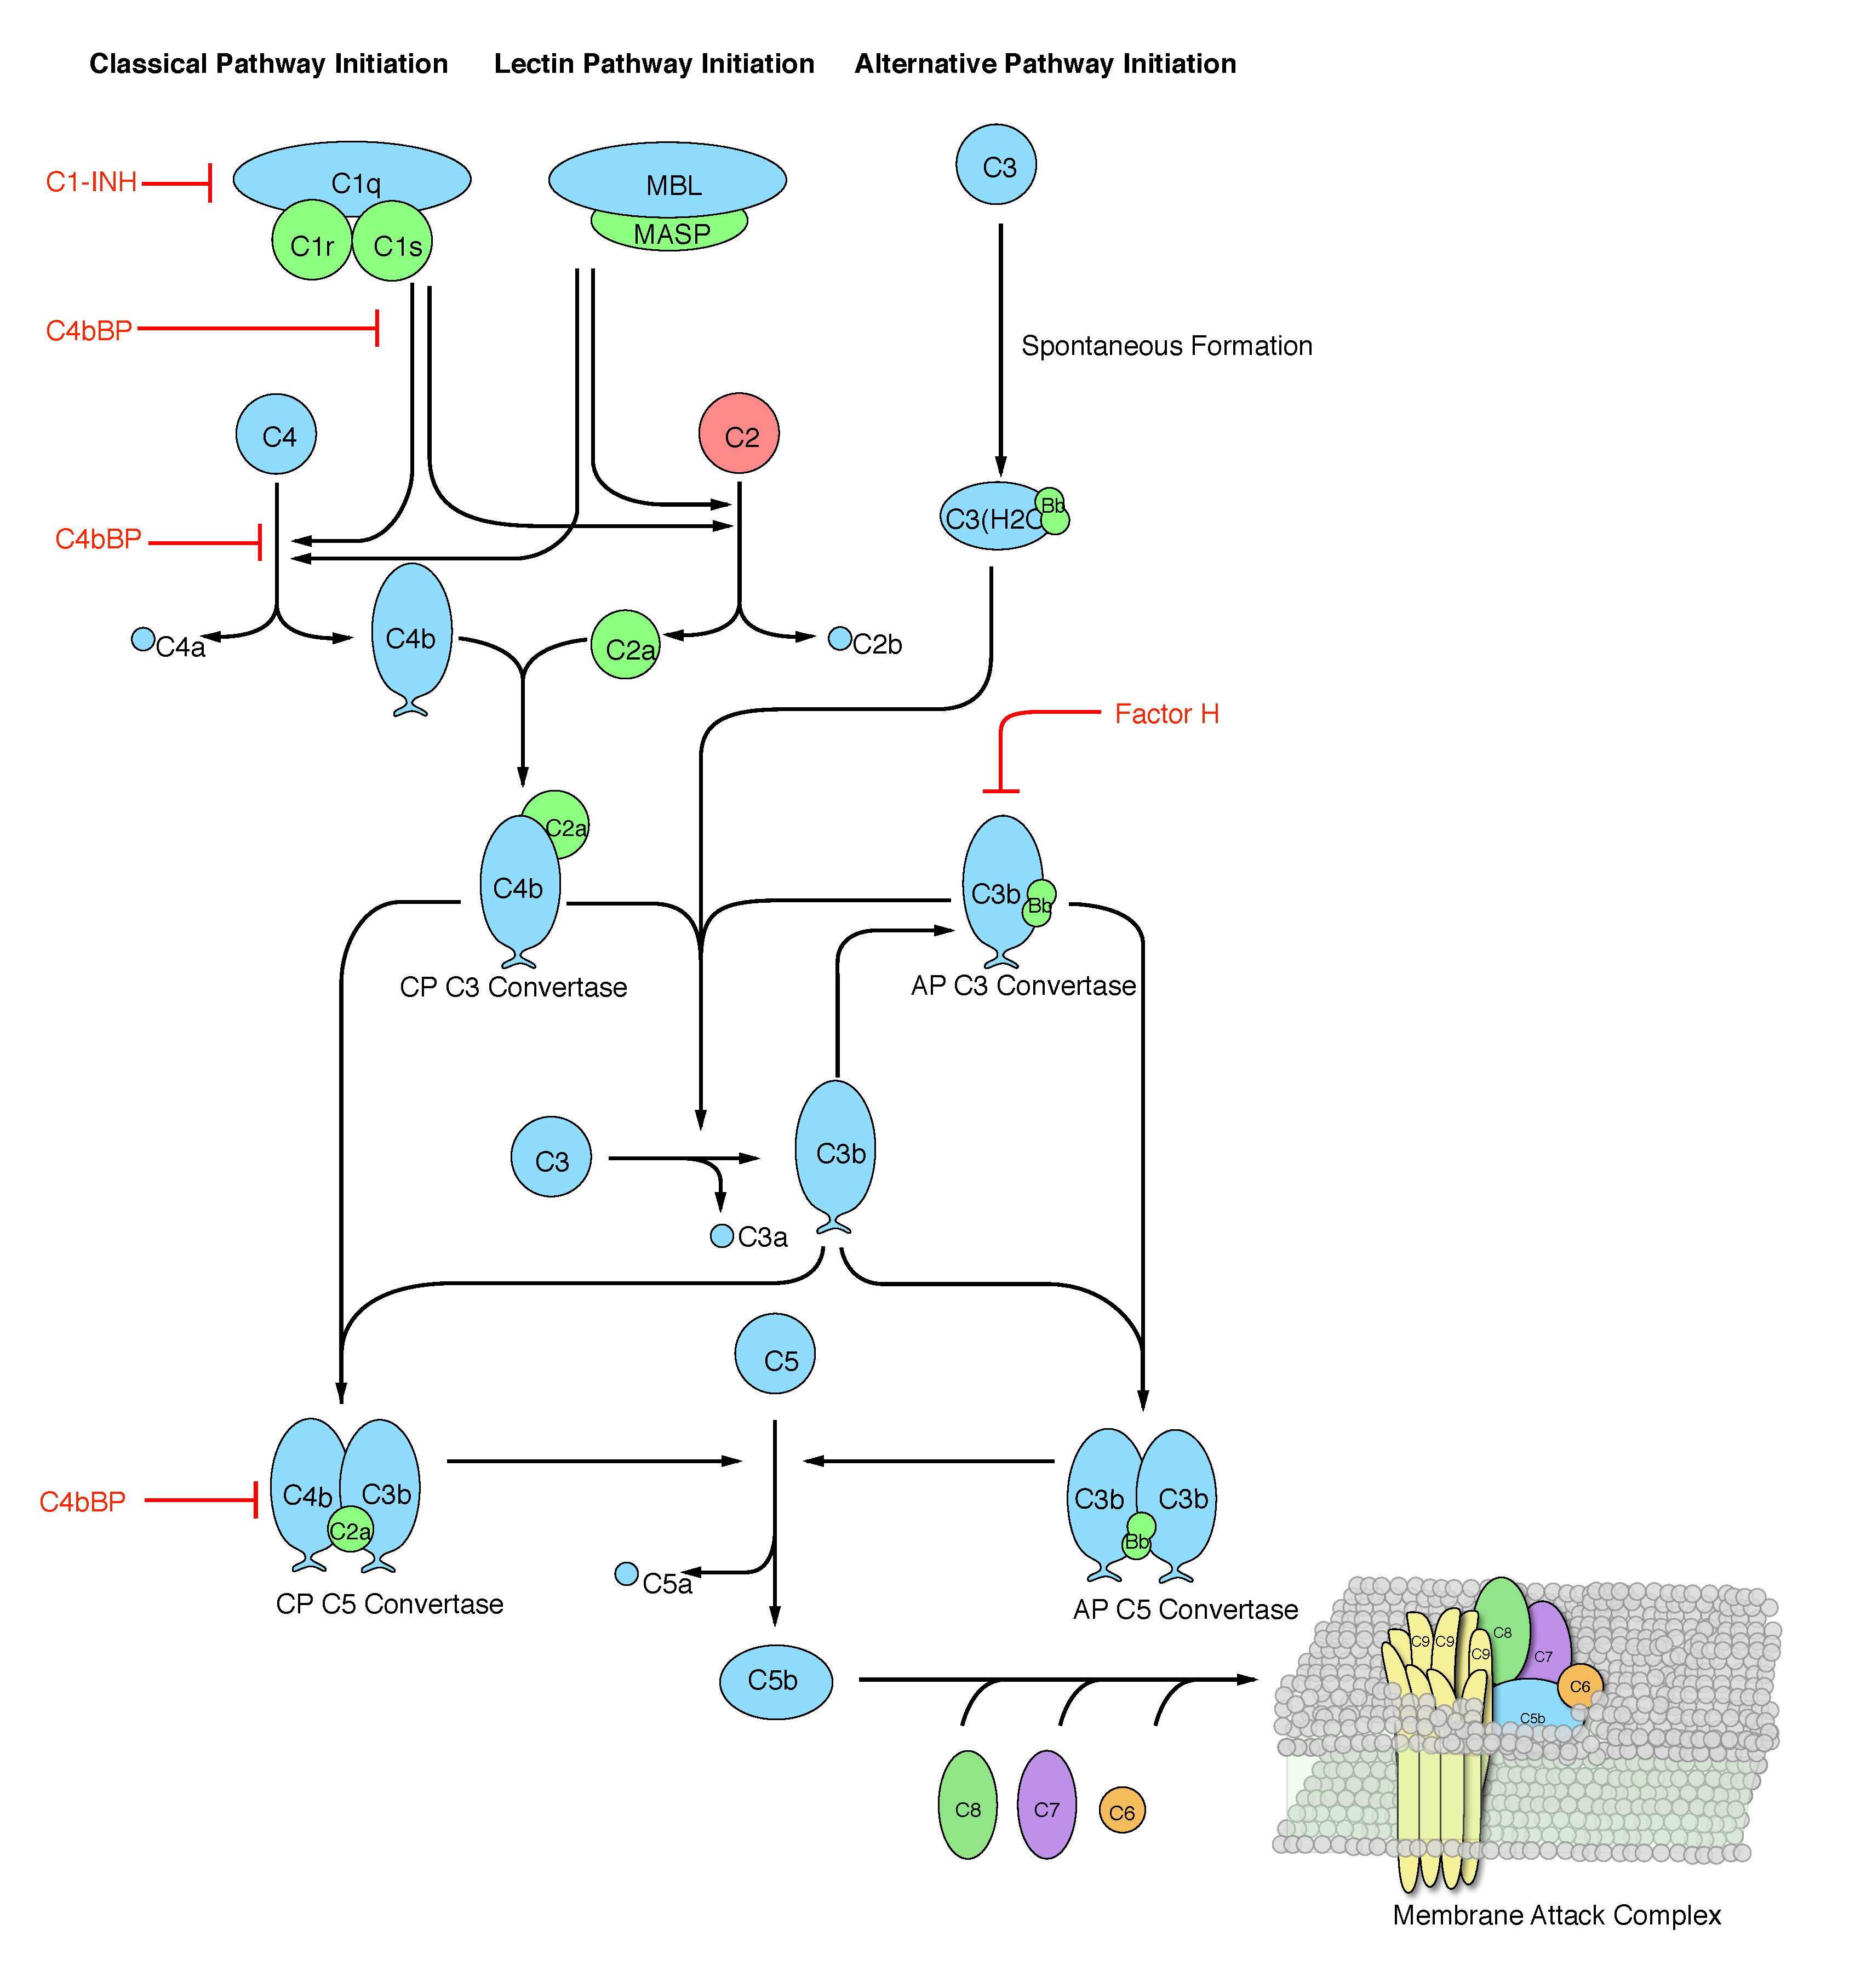
\includegraphics[width=1.0\textwidth]{./figs/Fig1_Schematic_v2.pdf}
\caption{Simplified schematic of the human complement system. The complement cascade is activated through any one, or more, of the three pathways:  the classical, the lectin, and the alternate pathways. The classical pathway is activated by the binding of C1 complex through the C1q subunit to the IgG or IgM immune complex.  This binding leads to conformational changes in the C1 complex that leads to the activation of C1r and C1s subunits. Activated C1-antibody complex cleaves C4 and C2 to form the classical C3 convertase. The lectin pathway is initiated by the binding mannose-binding lectins (MBL) and ficolins to carbohydrate moieties on the pathogen surfaces. This results in the formation mannose-binding lectin-associated serine proteases (MASPs). The MBL-MASP complex cleaves C4 and C2 to form the lectin C3 convertase. The alternative pathway is activated through a spontaneous tick-over mechanism by the hydrolysis of C3 to form fluid phase C3 convertase. The C3 convertases  cleaves C3 into C3a, and C3b. C3b combines with C4b and C2a to form classical C5 convertase (C4bC3aC3b). The C3b binds with Factor B to form the alternate C5 convertase (C3bBbC3b) . The C5 convertases cleave C5 into C5a, and C5b that undergoes a series of reactions to form the membrane attack complex (MAC).}\label{fig-schematic}
\end{figure}



\begin{figure}[h]
\centering
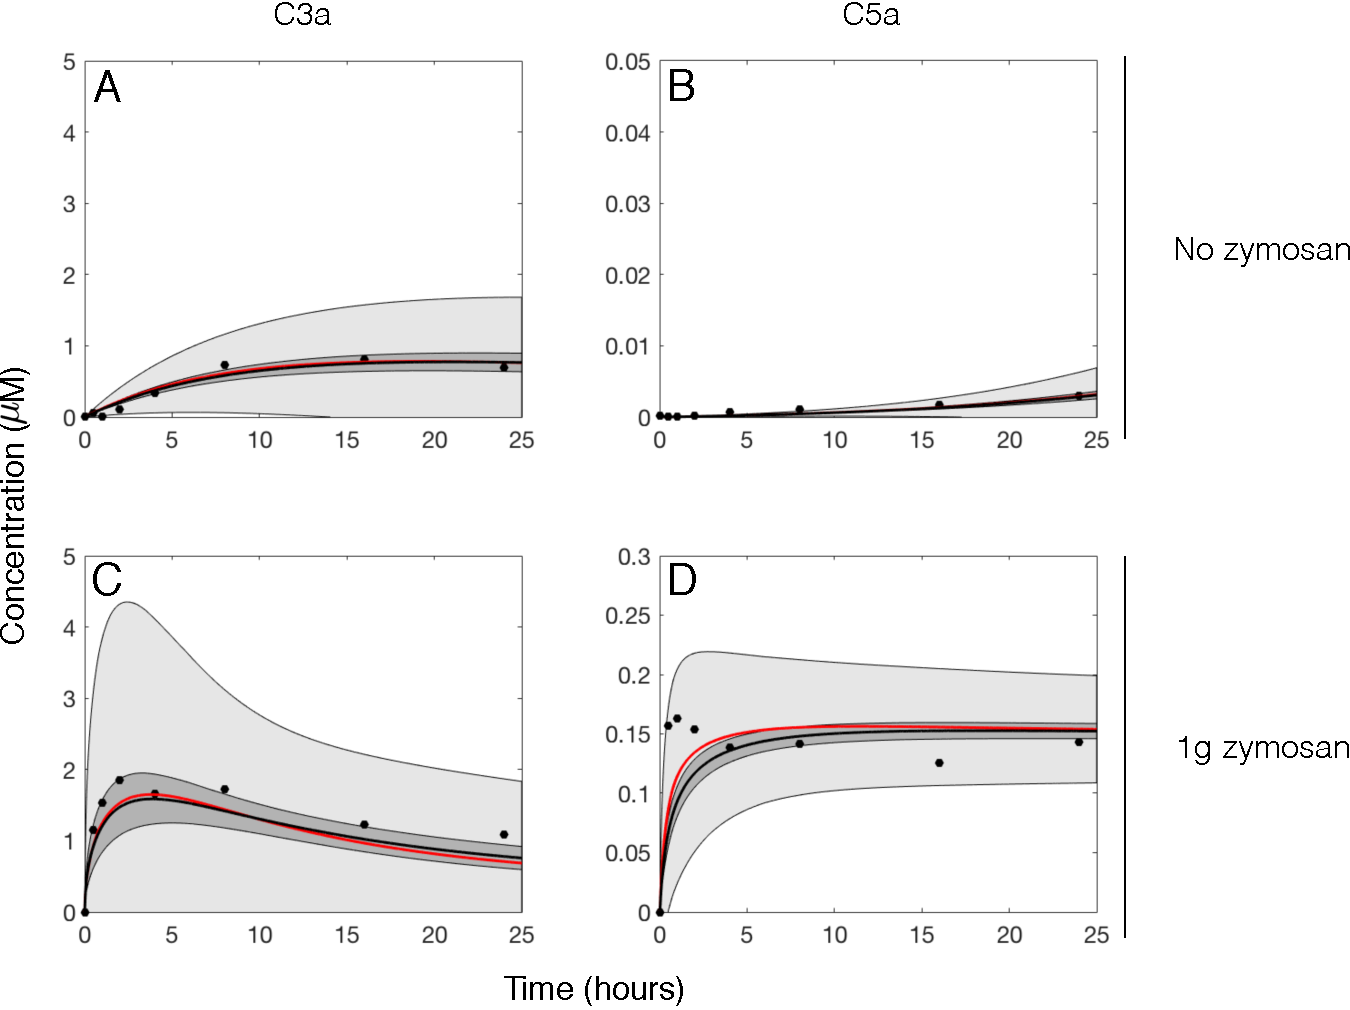
\includegraphics[width=1.0\textwidth]{./figs/Figure2_Fits_final.pdf}
\caption{Reduced order complement model training simulations. Reduced order complement model parameters were estimated using Dynamic Optimization with Particle Swarms (DOPS). The model was trained against experimental data from Shaw and co-workers \cite{morad2015time} in the presence and absence of zymosan. The model was trained using C3a and C5a data generated from the alternative pathway (\textbf{A}--\textbf{B}) and lectin initiated pathway with 1g zymosan (\textbf{C}--\textbf{D}). The solid red line shows the simulation with the best-fit parameter, the solid black lines show the simulated mean value of C3a or C5a for 50 independent particles. The  dark shaded region denotes 99 \% confidence interval of the simulated mean concentrations of C3a or C5a , while the light shaded region is the 99 \% confidence interval of the best prediction. All initial concentrations of complement proteins are at human serum levels unless otherwise noted.}\label{fig-fit}
\end{figure}

\begin{figure}[h]
\centering
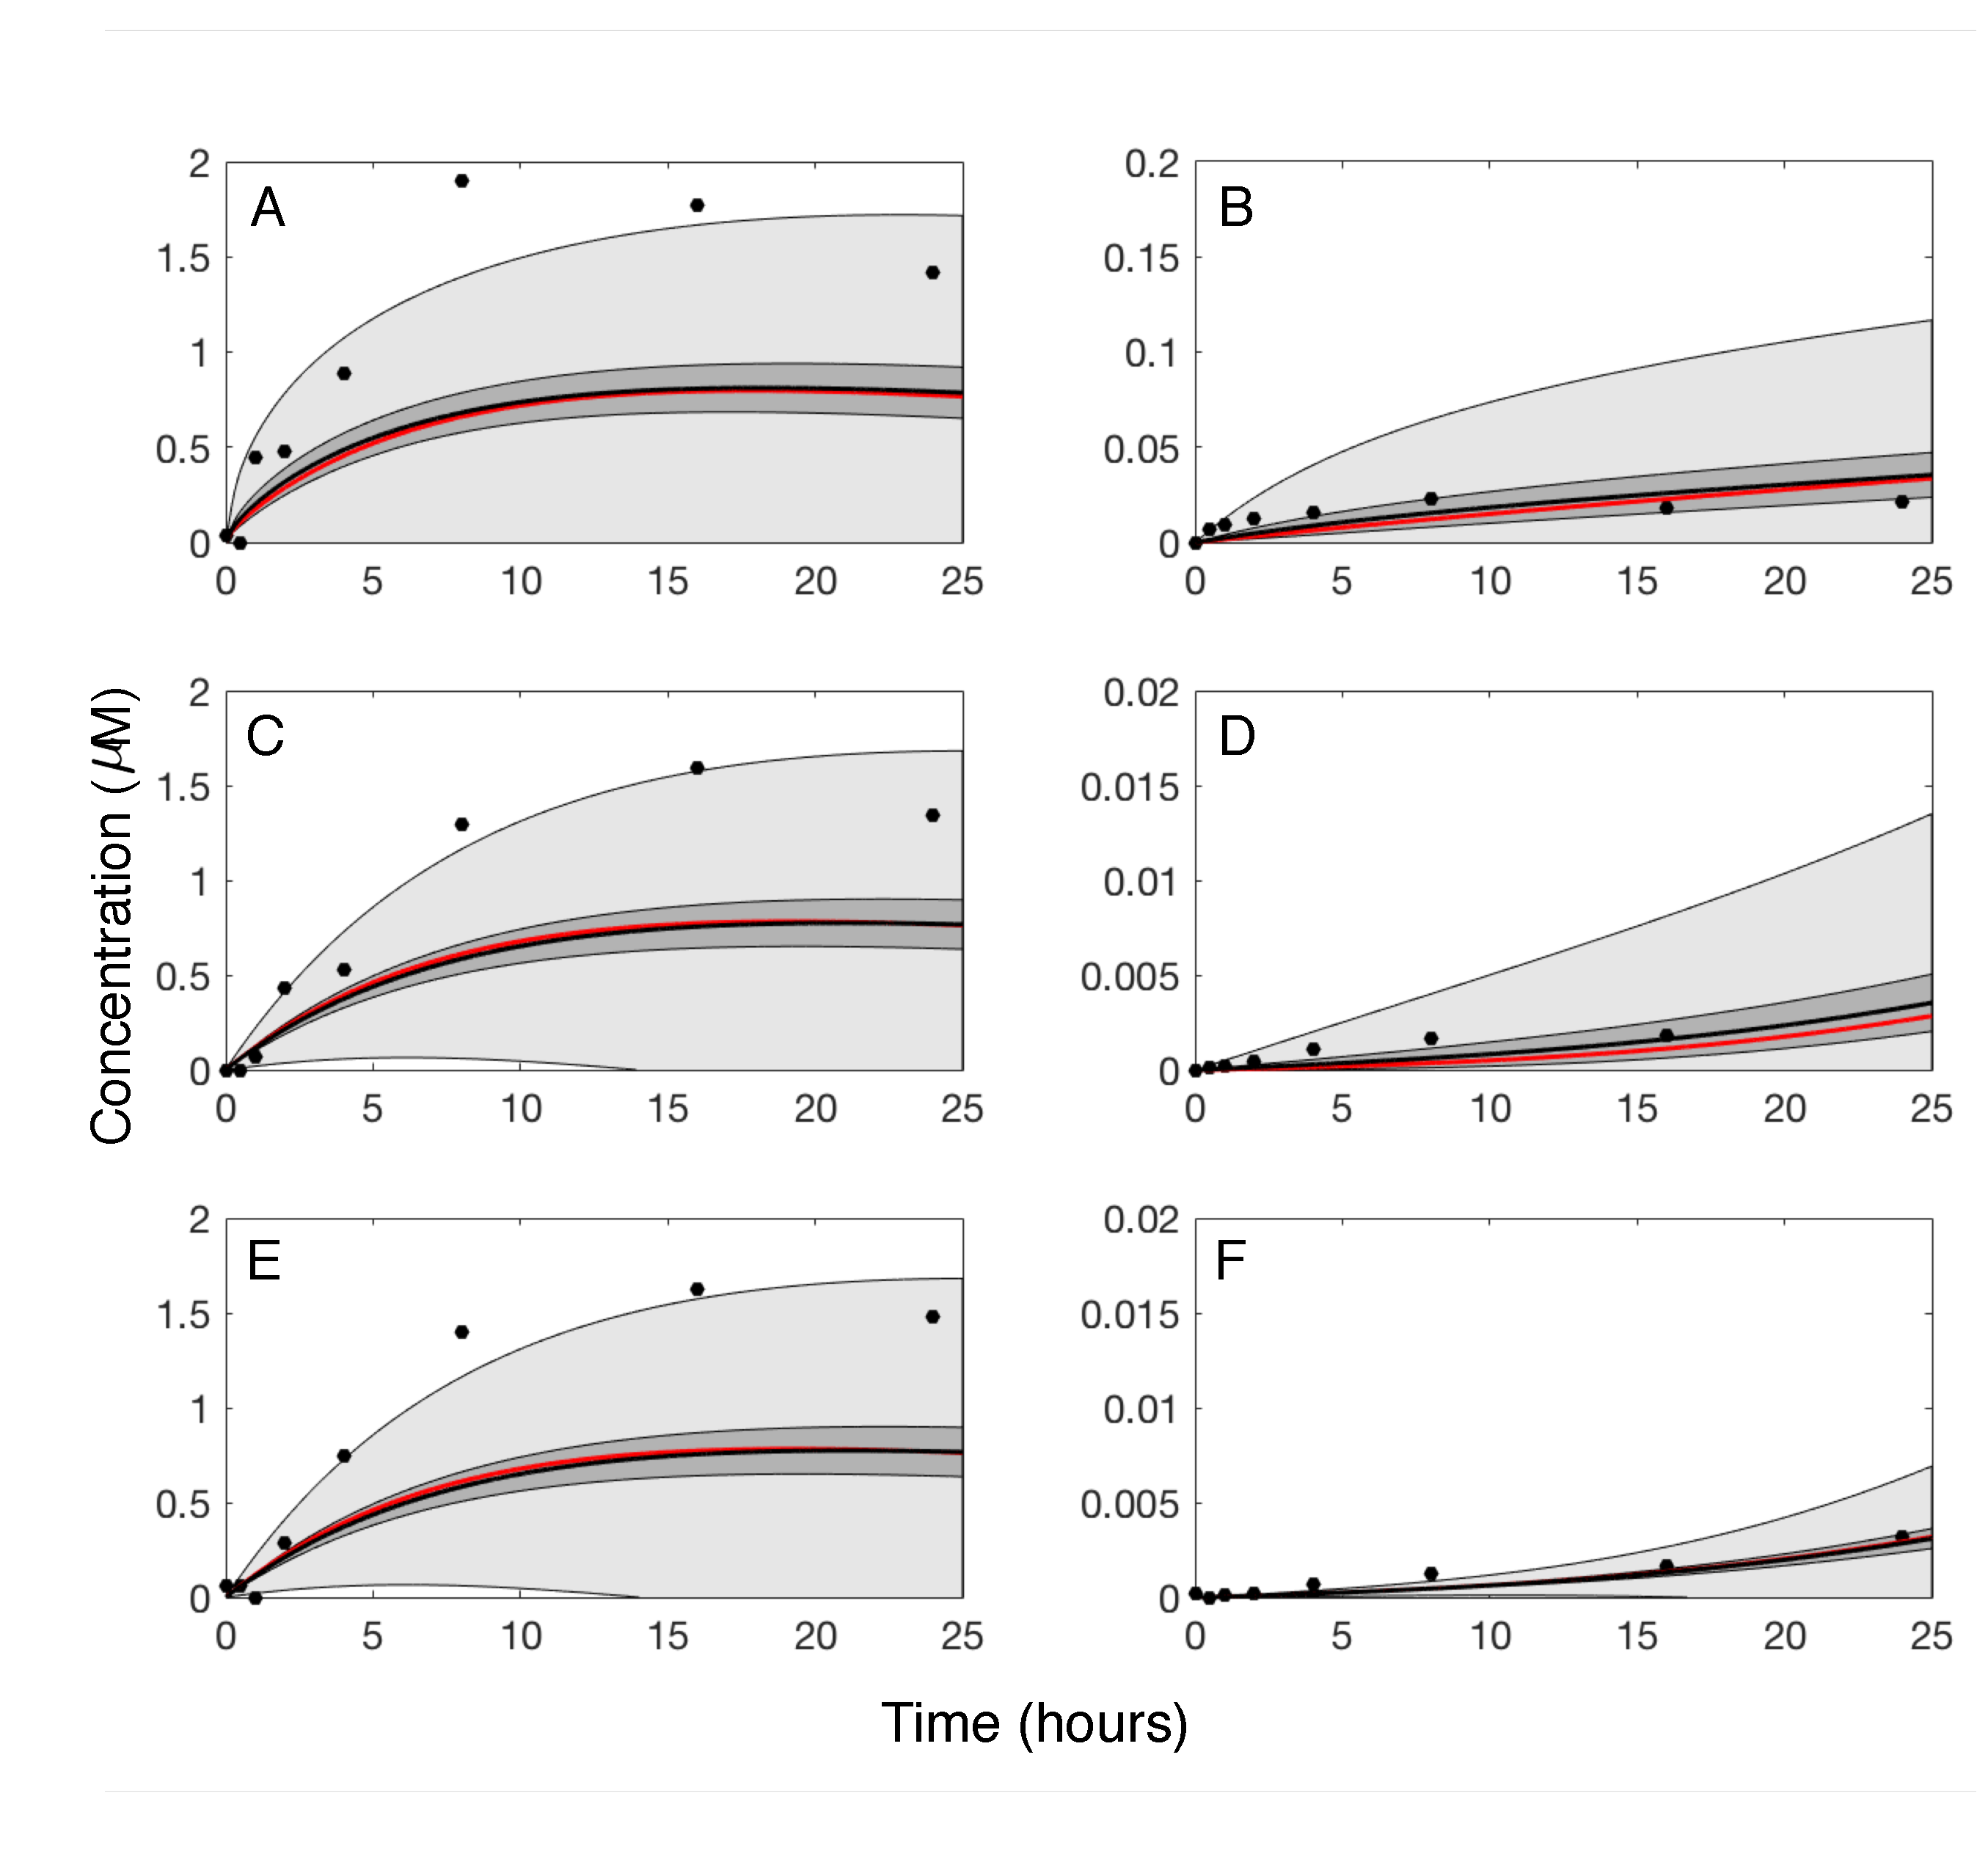
\includegraphics[width=1.0\textwidth]{./figs/Figure3_predictions_final.pdf}
\caption{Reduced order complement model predictions vs experimental data for C3a and C5a generated in the lectin pathway. The reduced order coagulation model parameter estimates were tested against data not used during model training. Simulations of C3a and C5a generated in the lectin pathway using different levels of zymosan ($0.1$, $0.01$, and $0.001$ grams of zymosan) were compared with the corresponding experimental data (\textbf{A}--\textbf{F}). The solid red line shows the simulation with the best-fit parameter, the solid black lines show the simulated mean value of C3a or C5a for 50 independent particles. The shaded region denotes 99 \% confidence interval of the simulated mean concentrations of C3a or C5a, while the light shaded region is the 99 \% confidence interval of the best prediction. All initial concentrations of complement proteins are at human serum levels unless otherwise noted.
}\label{fig-prediction}
\end{figure}

%\begin{figure}[h]
%\centering
%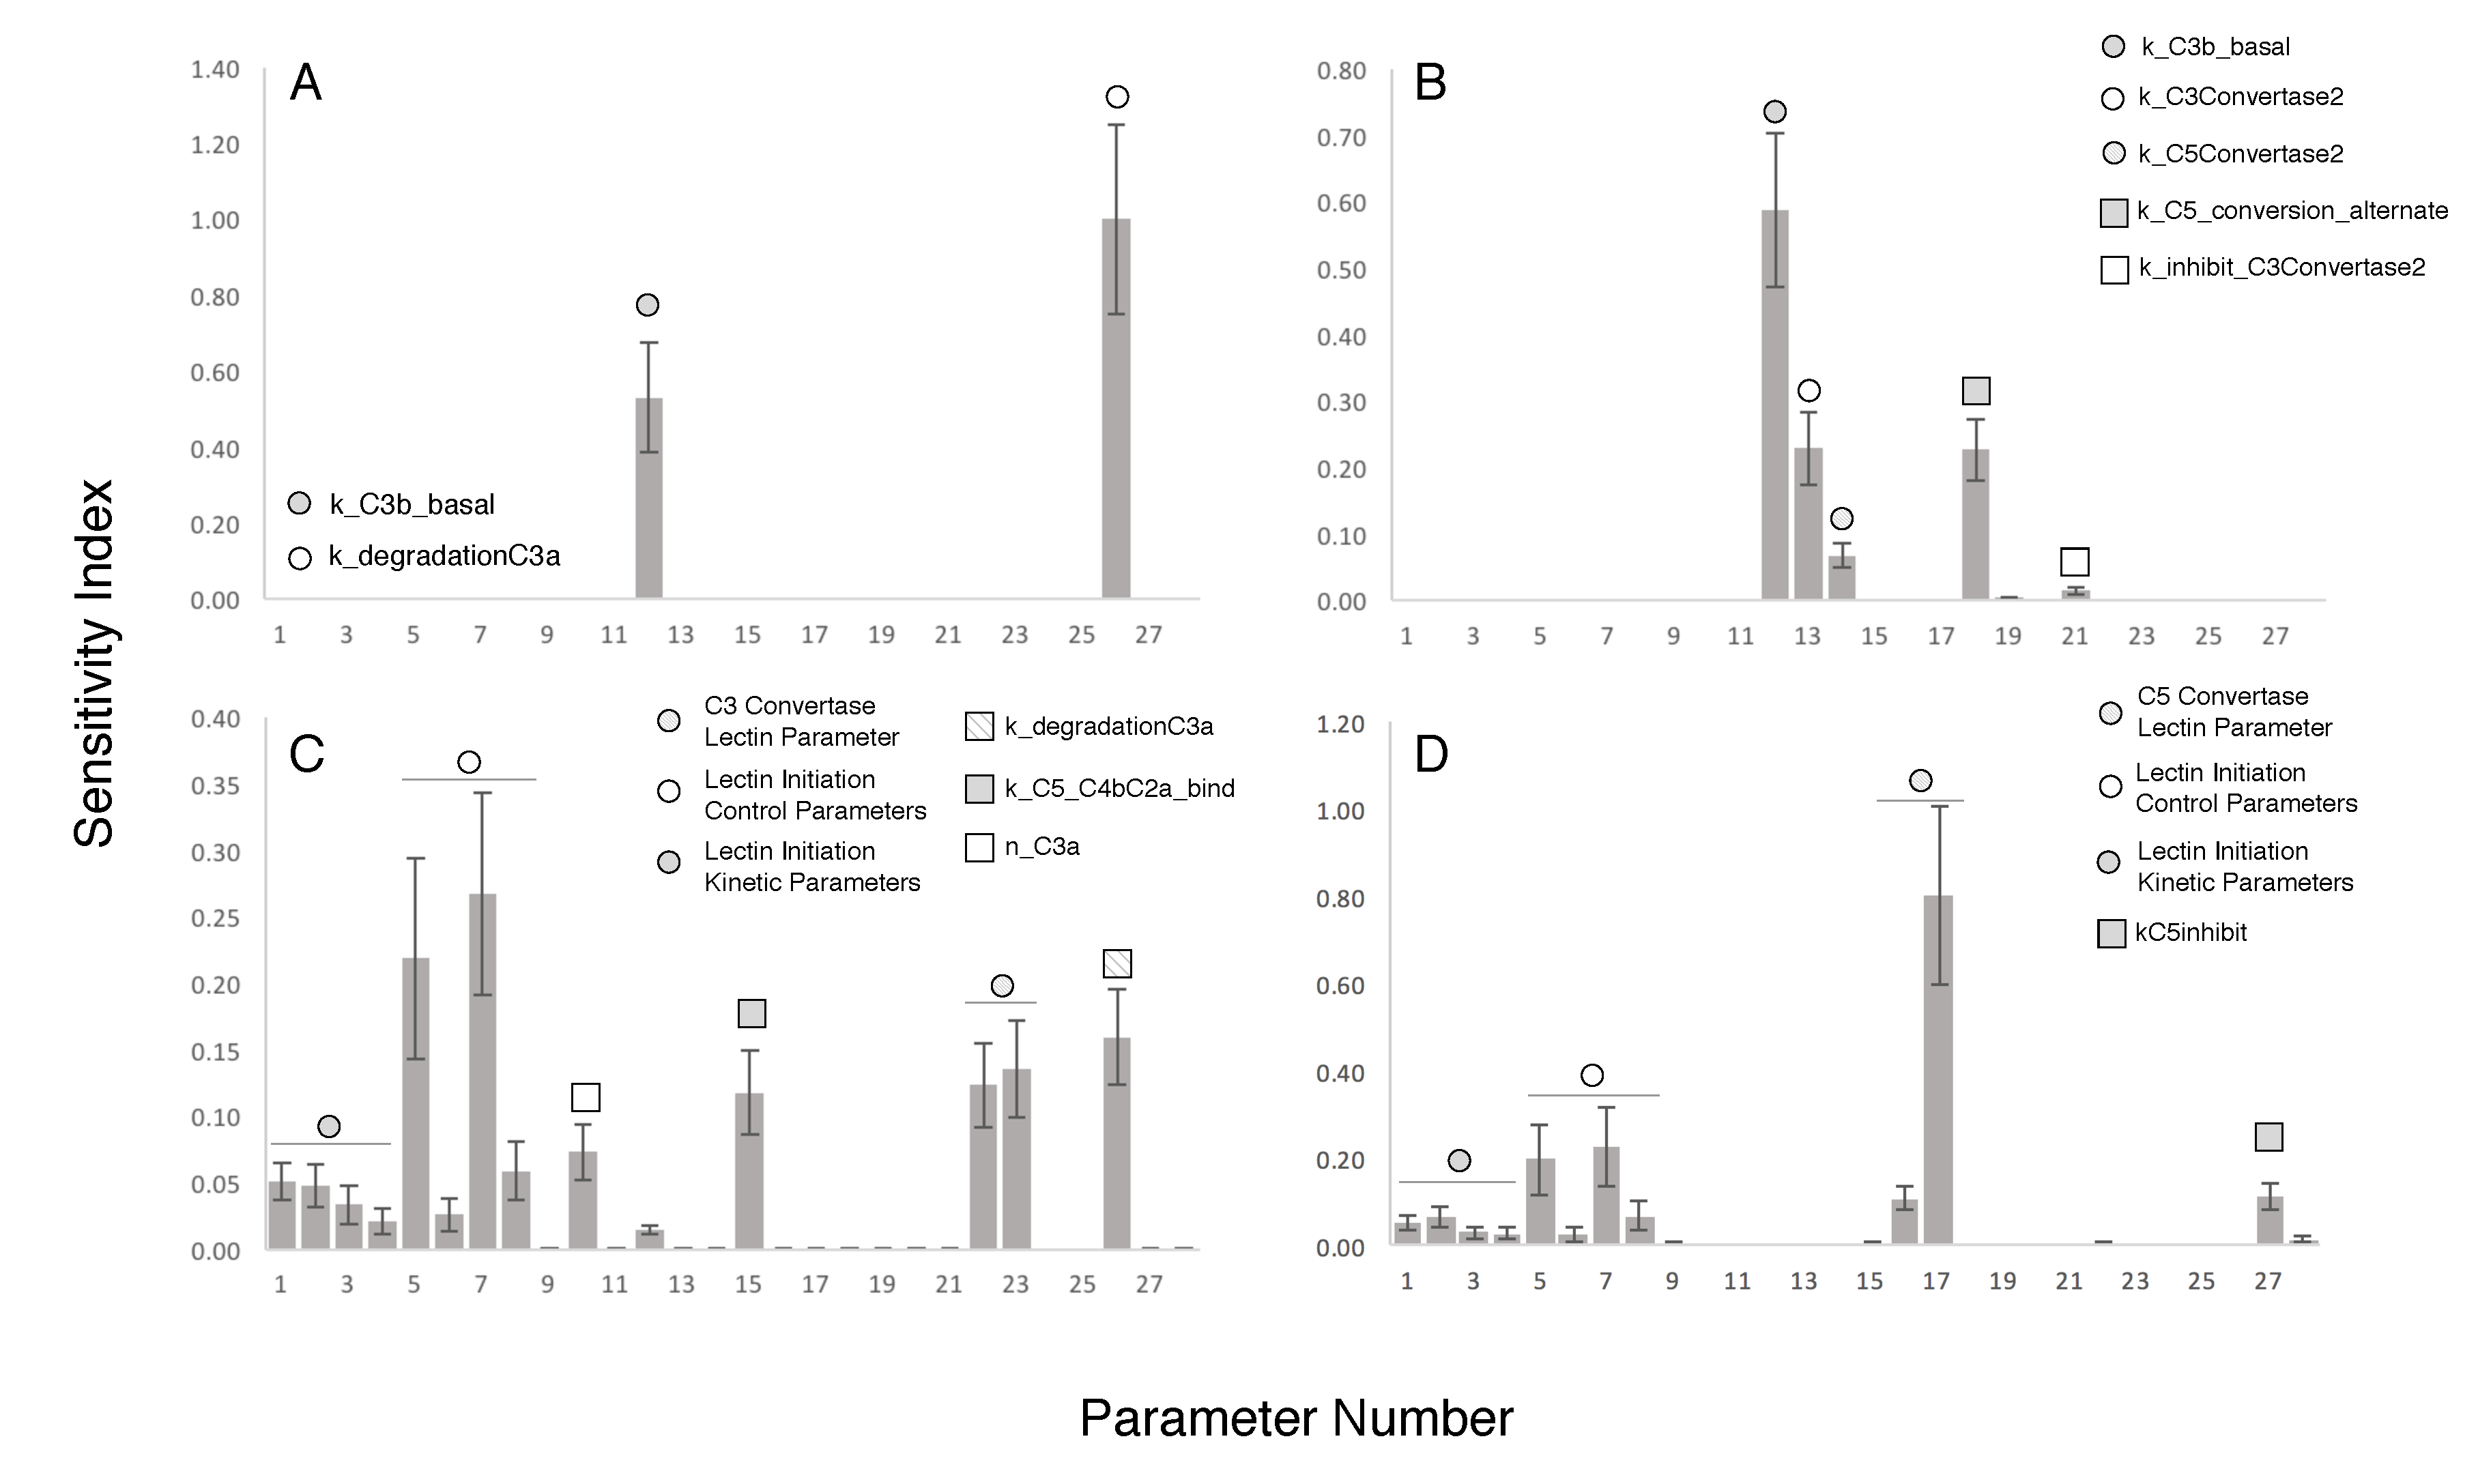
\includegraphics[width=1.0\textwidth]{./figs/Figure4_Sensitivity_Analysis_may25.pdf}
%\caption{Sobol's sensitivity analysis of the reduced order complement model with respect to the modeling parameters.  Sensitivity analysis was conducted on the four cases we used to train our model: (A) C3a at 0 zymosan, (B) C5a 0 zymosan, (C) C3a 1 g zymosan, and (D) C5a $1$ g zymosan. The bars denote total sensitivity index which includes local contribution of each parameter and global sensitivity of significant pairwise interactions. The error bars are the 95 percent confidence interval. $k$ represents association rate, $km$ denote Michaelis-Menten saturation constants, and $alpha$ and $n$ refers to the exponentials of the control functions.}\label{fig-SA}
%\end{figure}

\begin{figure}[h]
\centering
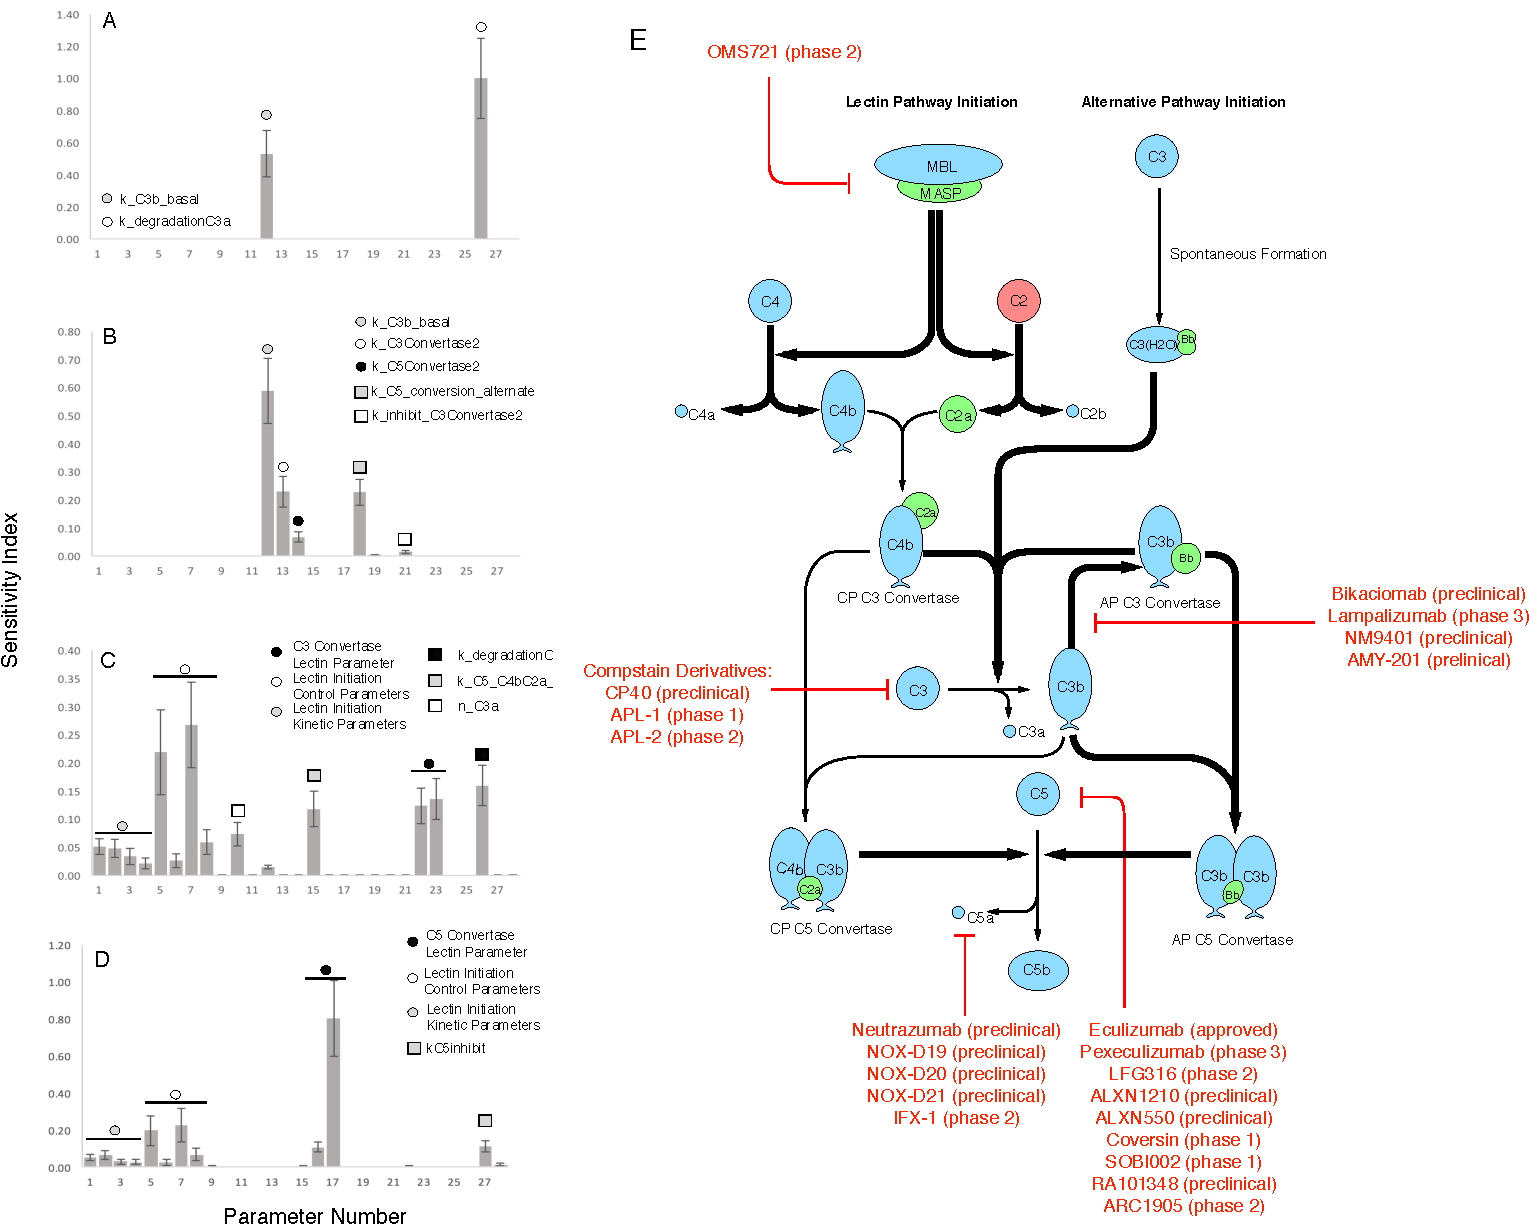
\includegraphics[width=1.0\textwidth]{./figs/Figure4_SEN_v2.pdf}
\caption{Sobol's sensitivity analysis of the reduced order complement model with respect to the modeling parameters.  Sensitivity analysis was conducted on the four cases we used to train our model: (A) C3a at 0g zymosan, (B) C5a 0g zymosan, (C) C3a 1g zymosan, and (D) C5a 1g zymosan. The bars denote total sensitivity index which includes local contribution of each parameter and global sensitivity of significant pairwise interactions. The error bars are the 95 percent confidence interval. Pathways controlled by the sensitivity parameters (E): Bold black lines indicates the pathway is governed by one or more sensitive parameters and the red lines shows some of the current therapeutics targets. Red indicates current complement therapeutics. }\label{fig-SA}
\end{figure}

\begin{figure}[h]
\centering
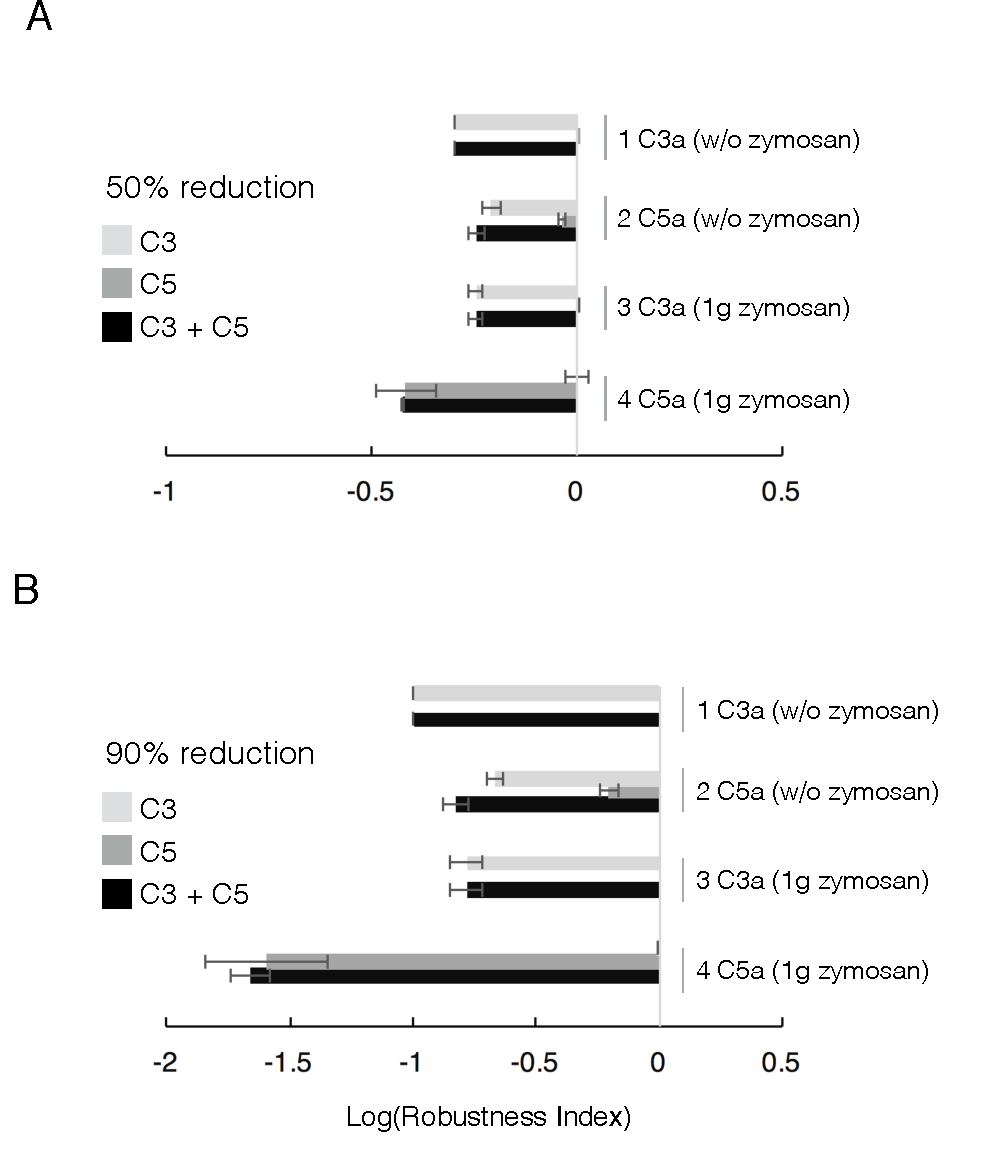
\includegraphics[width=1.0\textwidth]{./figs/Figure5_RobustnessAnalysis_v2.pdf}
\caption{Robustness analysis of the reduced order complement model with respect to the C3 and C5 initial concentrations using 50 parameter sets.  Robustness analysis was conducted on the four cases we used to train our model, C3a alternate (0 zymosan), C5a alternate (0 zymosan),  C3a lectin (1 g zymosan), and C5a lectin (1 g zymosan), by reducing the initial concentration of C3 and/or C5 by (A) 50 \% and (B) 90 \%. The bars denote robustness index which a measure of system changes from the perturbation of initial concentration that defined by the ratio of the area under the concentration curve of perturbed case and that of the unperturbed case. The error bars represent one standard deviation. At unity, the perturbed initial concentration has no impact on the measured output, and a robustness index lesser than or greater than one indicates a negative or positive relation between the perturbed initial concentration and the measured output respectively.}\label{fig-robustness-analysis}
\end{figure}


% \begin{figure}[h]
% \centering
% 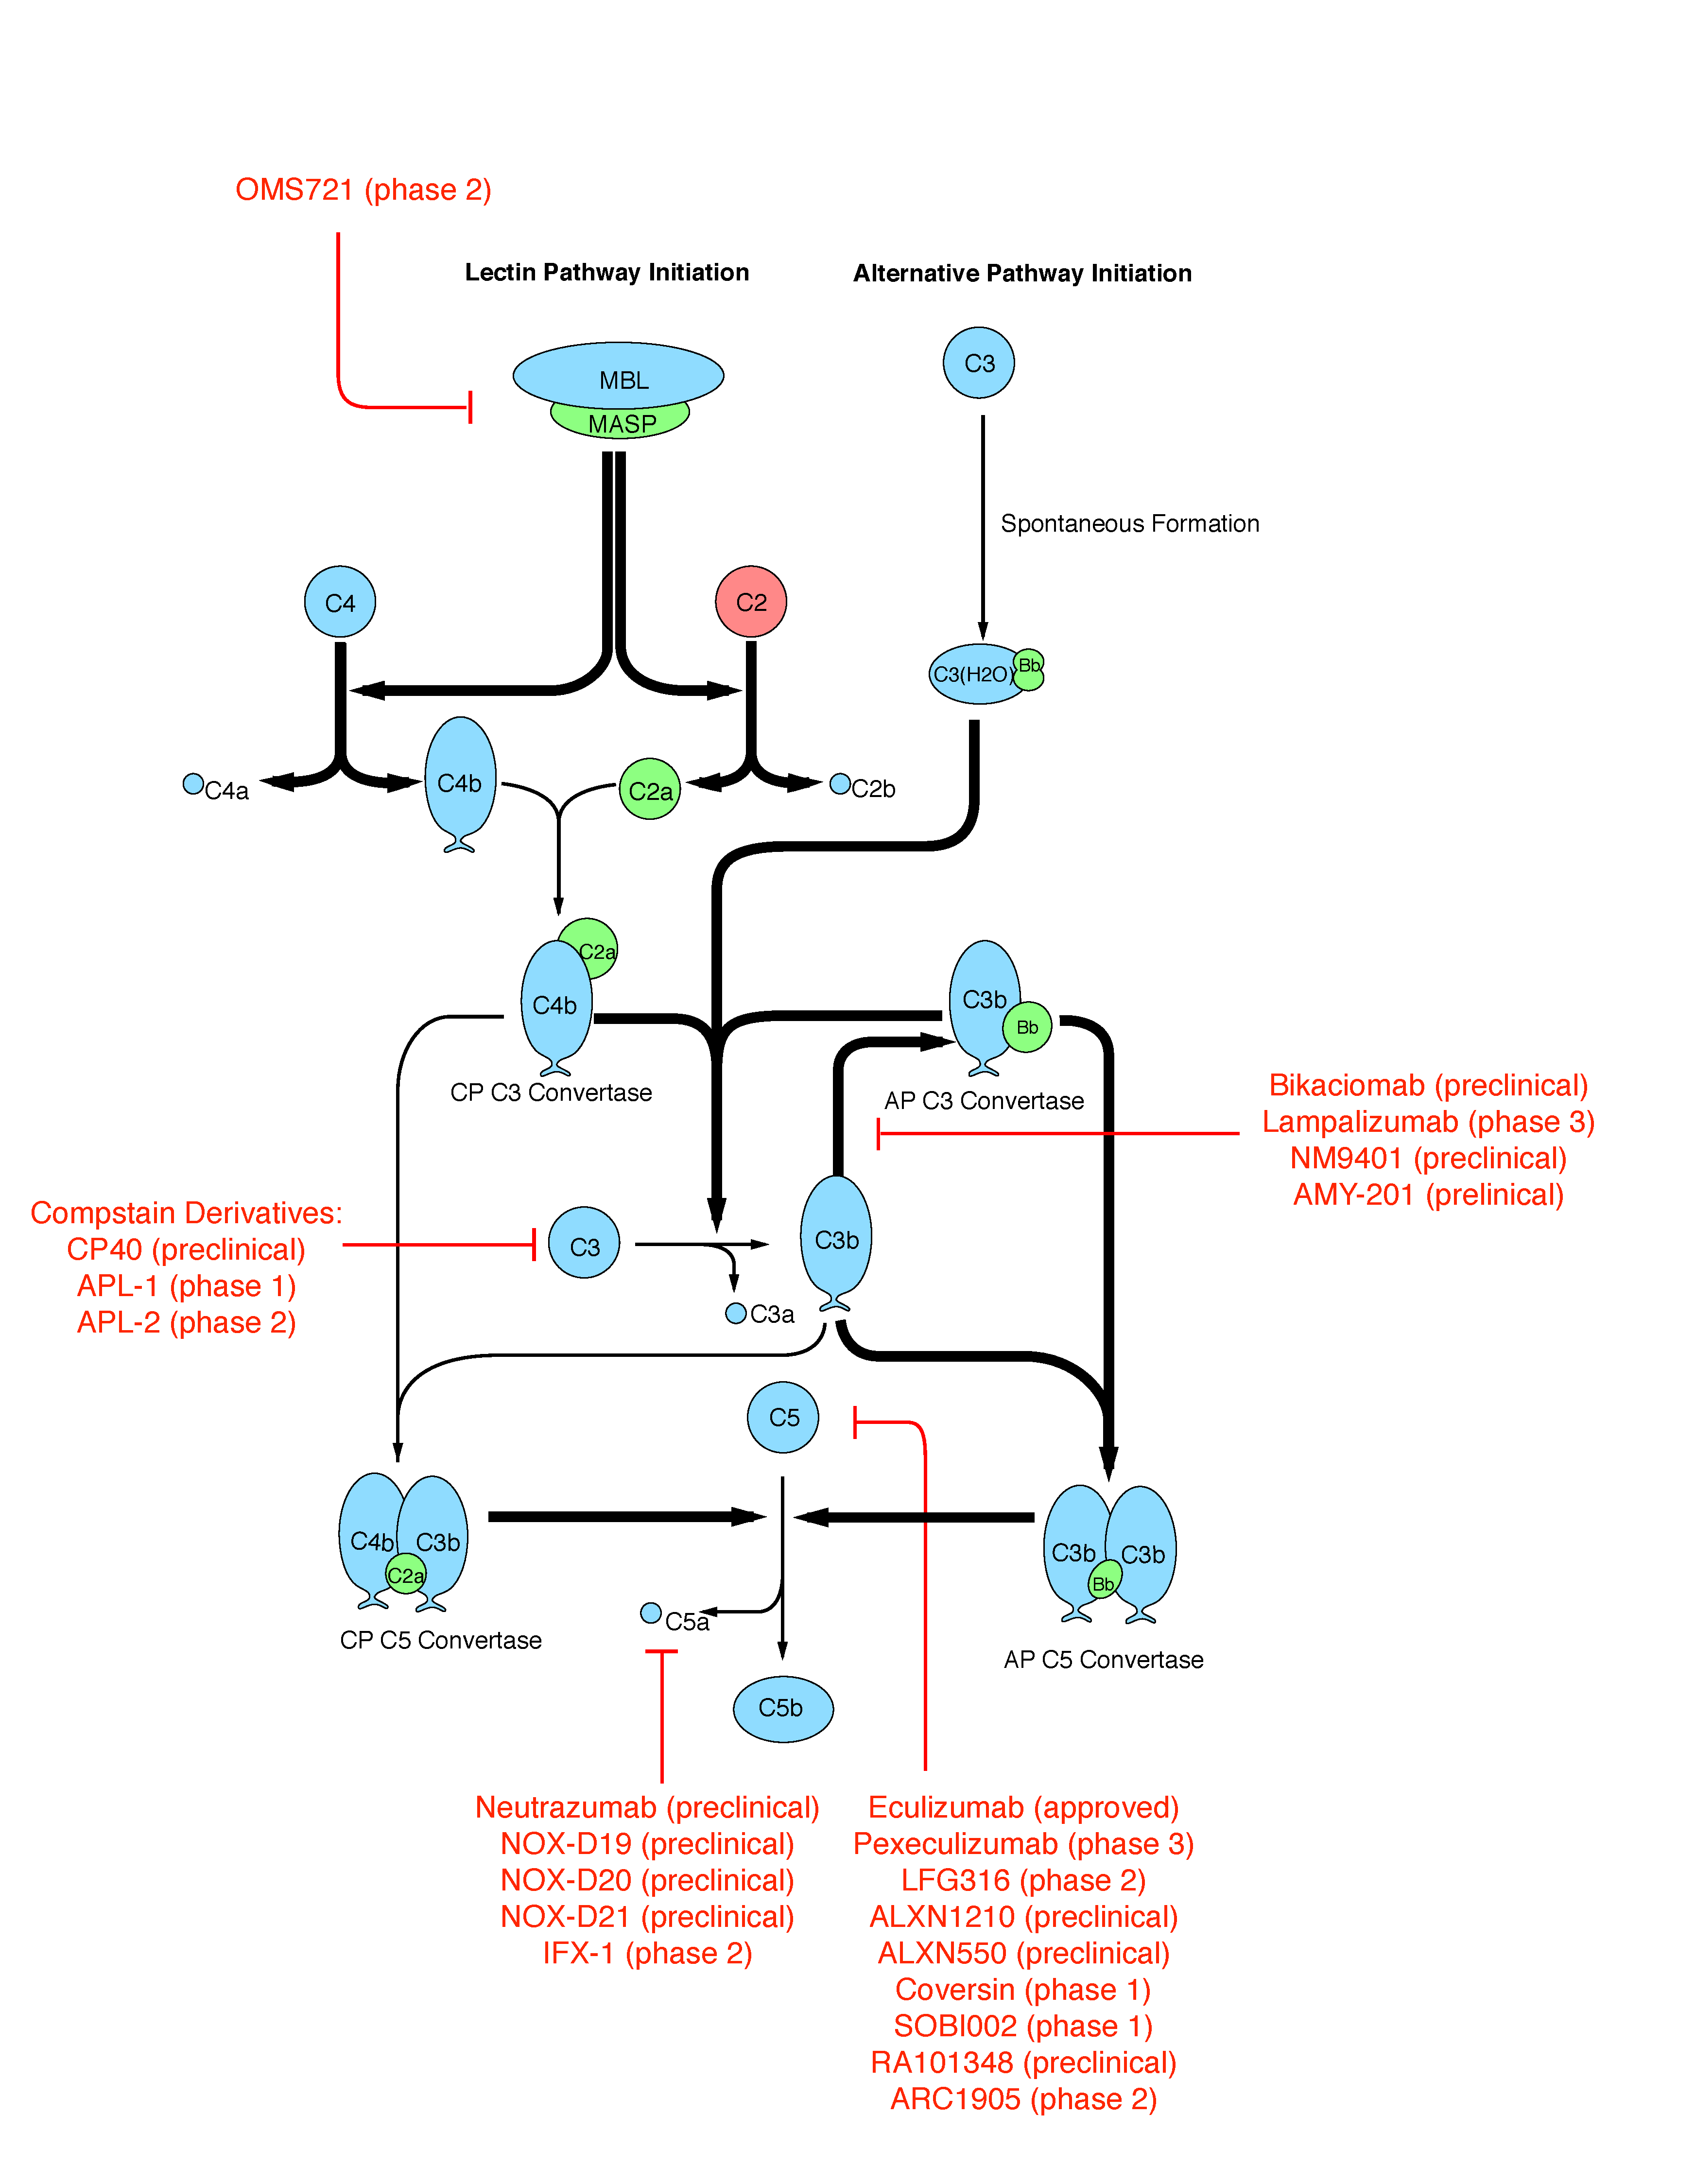
\includegraphics[width=1.0\textwidth]{./figs/Figure6_target.pdf}
% \caption{ The figure graphically illustrates some of the current complement therapeutics and their targets within our network. A vast majority of the drugs target the terminal pathway by targeting C5 or C5a. Targeting C5 would reduce the formation of C5a and C5b, however targeting C5a directly would reduce the influence of the anaphylatoxin but still produce precursors for the MAC formation. A number of therapeutics also target C3 and the formation of AP C3 convertase through the inhibition of Factors B and D. Finally, very few drugs target complement initiation, this may be due to a need for balance between immunity and inflammation or other complement related diseases.
% }\label{fig-targets}
% \end{figure}


\clearpage

% Supplemental figures -
% Set the S-
\renewcommand\thefigure{S\arabic{figure}}
\renewcommand\thetable{T\arabic{table}}
\renewcommand\thepage{S-\arabic{page}}
\renewcommand\theequation{S\arabic{equation}}

% Reset the counters -
\setcounter{equation}{0}
\setcounter{table}{0}
\setcounter{figure}{0}
\setcounter{page}{1}


\section*{Supplemental materials.}
\subsection*{Model equations.}
The reduced-order complement model consisted of 18 ordinary differential equations, 12 rate equations, and two control equations:
\begin{eqnarray}
	\frac{dx_{1}}{dt} & =& - r_{1}f_{1} \\ 								%C4
	\frac{dx_{2}}{dt} &=& - r_{2}f_{2} \\  								%C2
	\frac{dx_{3}}{dt} &=&  r_{1}f_{1} \\ 								%C4a
	\frac{dx_{4}}{dt} &=& r_{1}f_{1} - r_{6} \\ 					%C4b
	\frac{dx_{5}}{dt} & = & r_{2}f_{2} - r_{6} \\ 					%C2a
	\frac{dx_{6}}{dt} &=& r_{2}f_{2} \\ 								%C2b
	\frac{dx_{7}}{dt} &=& r_{3} - r_{4} - r_{5}\\ 				%C3
	\frac{dx_{8}}{dt} &=& r_{3}  + r_{4} + r_{5}  - k_{deg,c3a}*C3a \\		%C3a
	\frac{dx_{9}}{dt} &=& r_{3}  + r_{4} + r_{5}  -  r_{7} \\		%C3b
	\frac{dx_{10}}{dt} &=& r_{6} - r_{10} -  r_{8} \\			%CP C3C
	\frac{dx_{11}}{dt} &=& r_{7} - r_{11} -  r_{9} \\			%AP C3C
	\frac{dx_{12}}{dt} &=& r_{10} - r_{14} \\							%CP C5C
	\frac{dx_{13}}{dt} &=& r_{10}  \\											%AP C5C
	\frac{dx_{14}}{dt} &=& - r_{12} - r_{13} \\								%C5
	\frac{dx_{15}}{dt} &=&  r_{12} + r_{13} - k_{deg,c5a} \\					%C5a
	\frac{dx_{16}}{dt} &=& r_{12} + r_{13} \\								%C5b
	\frac{dx_{17}}{dt} &=& - r_{8} - r_{14} \\  				         %C4BP
	\frac{dx_{18}}{dt} &=& - r_{9} \\									%Factor H
\end{eqnarray}where the rate equations are given by:
\begin{eqnarray}
	r_{1} &=& \frac{k_{i1}(C4)}{(K_{1s} + C4)} \\
	r_{2} &=& \frac{k_{2}(C2)}{(K_{2s} + C2)} \\
	f_{1} &=& \frac{Zymo^{\eta_{1}}}{(Zymo^{\eta_{1}} + \alpha_{1}^{\eta_{1}})} \\
	f_{2} &=& \frac{Zymo^{\eta_{2}}}{(Zymo^{\eta_{2}} + \alpha_{2}^{\eta_{2}})} \\
	r_{3} &=& k_{3}(C3) \\
	r_{4} &=& \frac{k_{4}(C3C_{L})(C3^{\eta_{3})}}{(K_{4s}^{\eta_{3}} + C3^{\eta_{3}})}  \\
	r_{5} &=& \frac{k_{5}(C3C_{A})(C3)}{(K_{5s} + C3)} \\
	r_{6} &=& k_{6}(C4b)(C2a) \\
	r_{7} &=& k_{7}(C4b)(C2a) \\
	r_{8} &=& k_{8}(C3C_{L})(C4b)(C4BP) \\
	r_{9} &=& k_{9}(C3C_{A})(FactorH) \\
	r_{10} &=& k_{10}(C3C_{L})(C3b) \\
	r_{11} &=& k_{11}(C3C_{A})(C3b) \\
	r_{12} &=& \frac{k_{12}(C5C_{L})(C5^{\eta_{4}})}{(K_{12s}^{\eta_{4}} + C5^{\eta_{4}})} \\
	r_{13} &=& \frac{k_{13}(C5C_{A})(C5)}{(K_{13s} + C5)} \\
	r_{14} &=& k_{14}(C5C_{L})(C4BP)
\end{eqnarray}

% Supplemental figures go here ...
%\begin{figure}[ht]
%\centering
%\includegraphics[width=1.00\textwidth]{./figs/<Filename>.pdf}
%\caption{Captiontext goes here}
%}\label{fig:<label_name>}
%\end{figure}

\end{document}
